\chapter{Supplementary material}
\begin{figure}[h!]
    \centering
    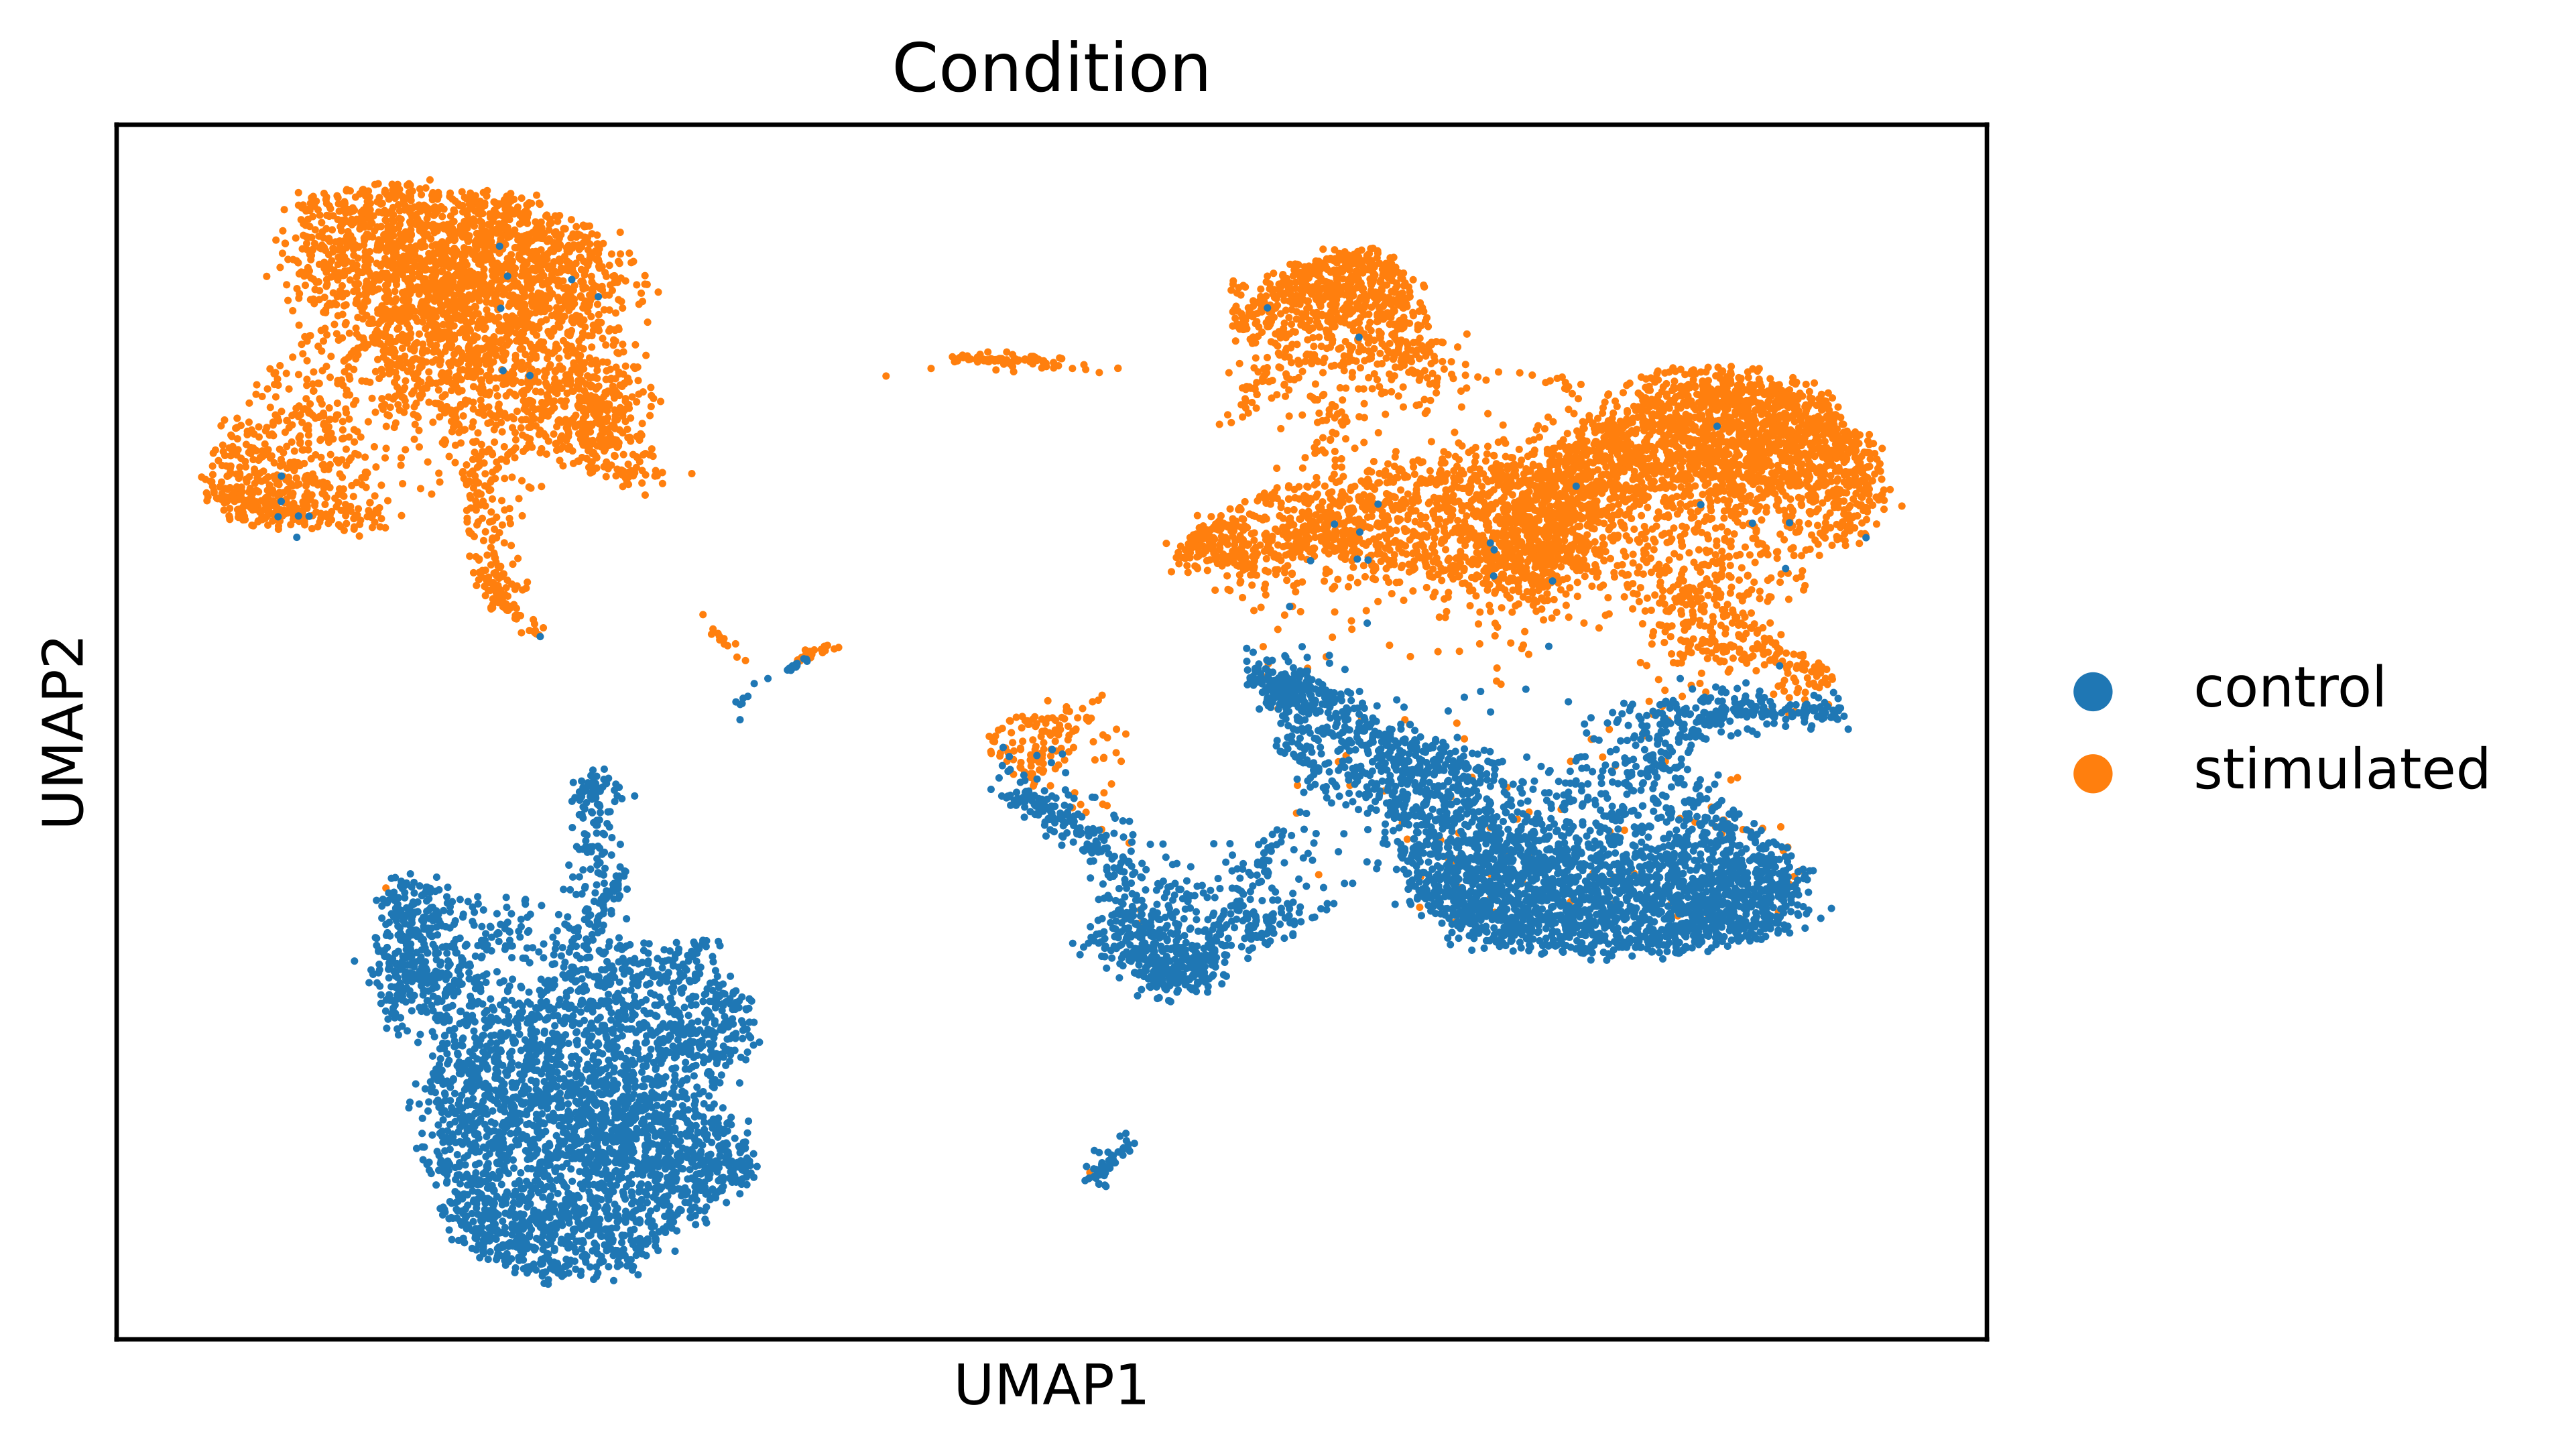
\includegraphics[scale=0.50]{reproducibility/reproducibility_appx.png}
    \caption{\small{\textbf{Reproduction of results in VEGA paper} | We reproduced the PBMCs analysis using VEGA and the Reactome pathways as the prior. The UMAP plot shows cells were nicely separated based on their treatment conditions.}}
    \label{fig:reproducibility_appx}
\end{figure}

\begin{figure}[h!]
    \centering
    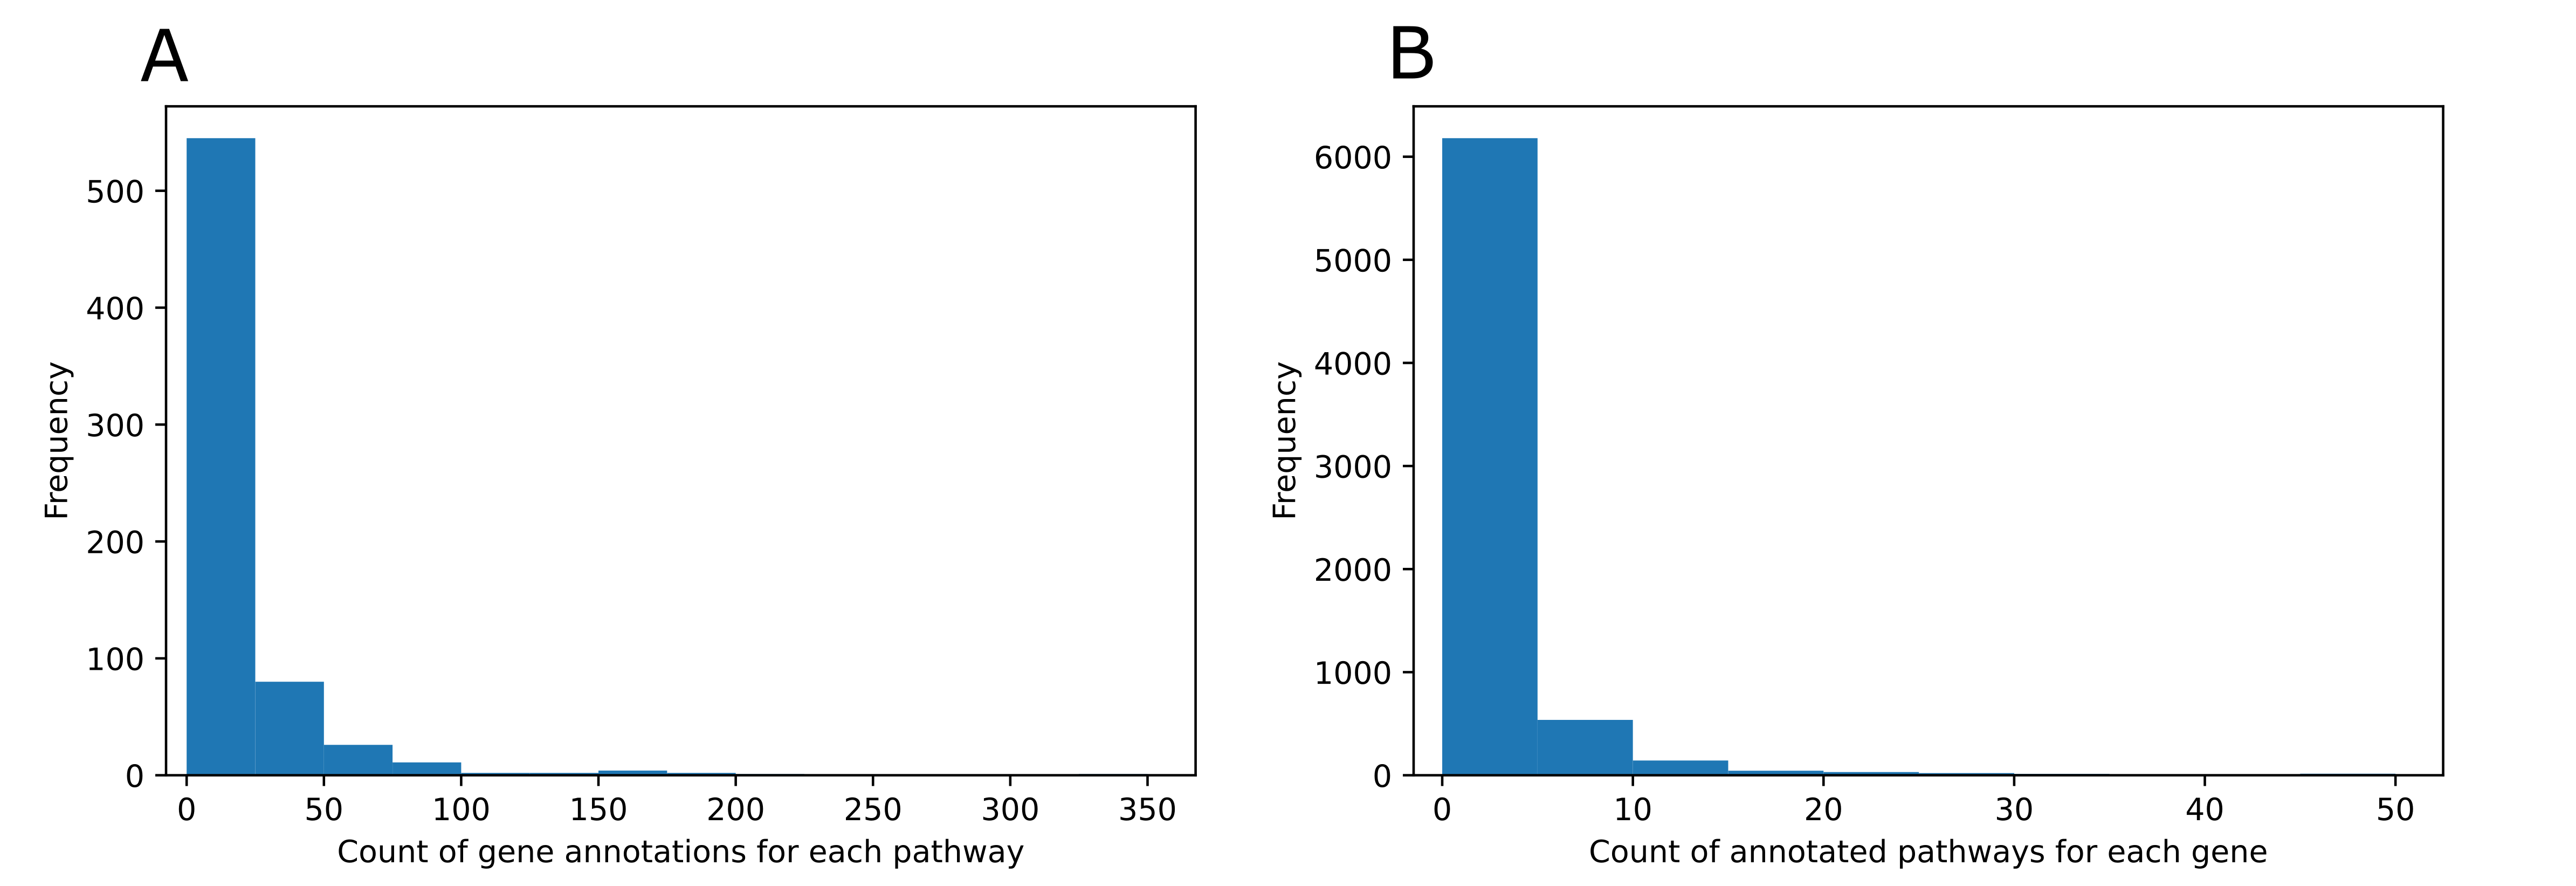
\includegraphics[scale=0.7]{reproducibility/stability_appx.png}
    \caption{\small{The caption is on the next page page.}}
    \label{fig:stability_appx}
\end{figure}

\addtocounter{figure}{-1}
\begin{figure}[t!]
    \caption{\small{\textbf{Outline of decoder wiring using PBMCs dataset} | \textbf{(A)} The x-axis indicates the number of genes each GMV connects to and the y-axis indicates the frequency of each case. We found that, unexpectedly, a high proportion of genes (5086 out of 6998) were not annotated in any of the Reactome pathways, which means the reconstructions of these 5086 genes were dependent only on one additional fully connected node in the latent space. \textbf{(B)} The x-axis indicates the number of GMVs each gene in the output layer connects to.}}
\end{figure}

\begin{figure}[b!]
    \centering
    \hspace*{-4mm}
    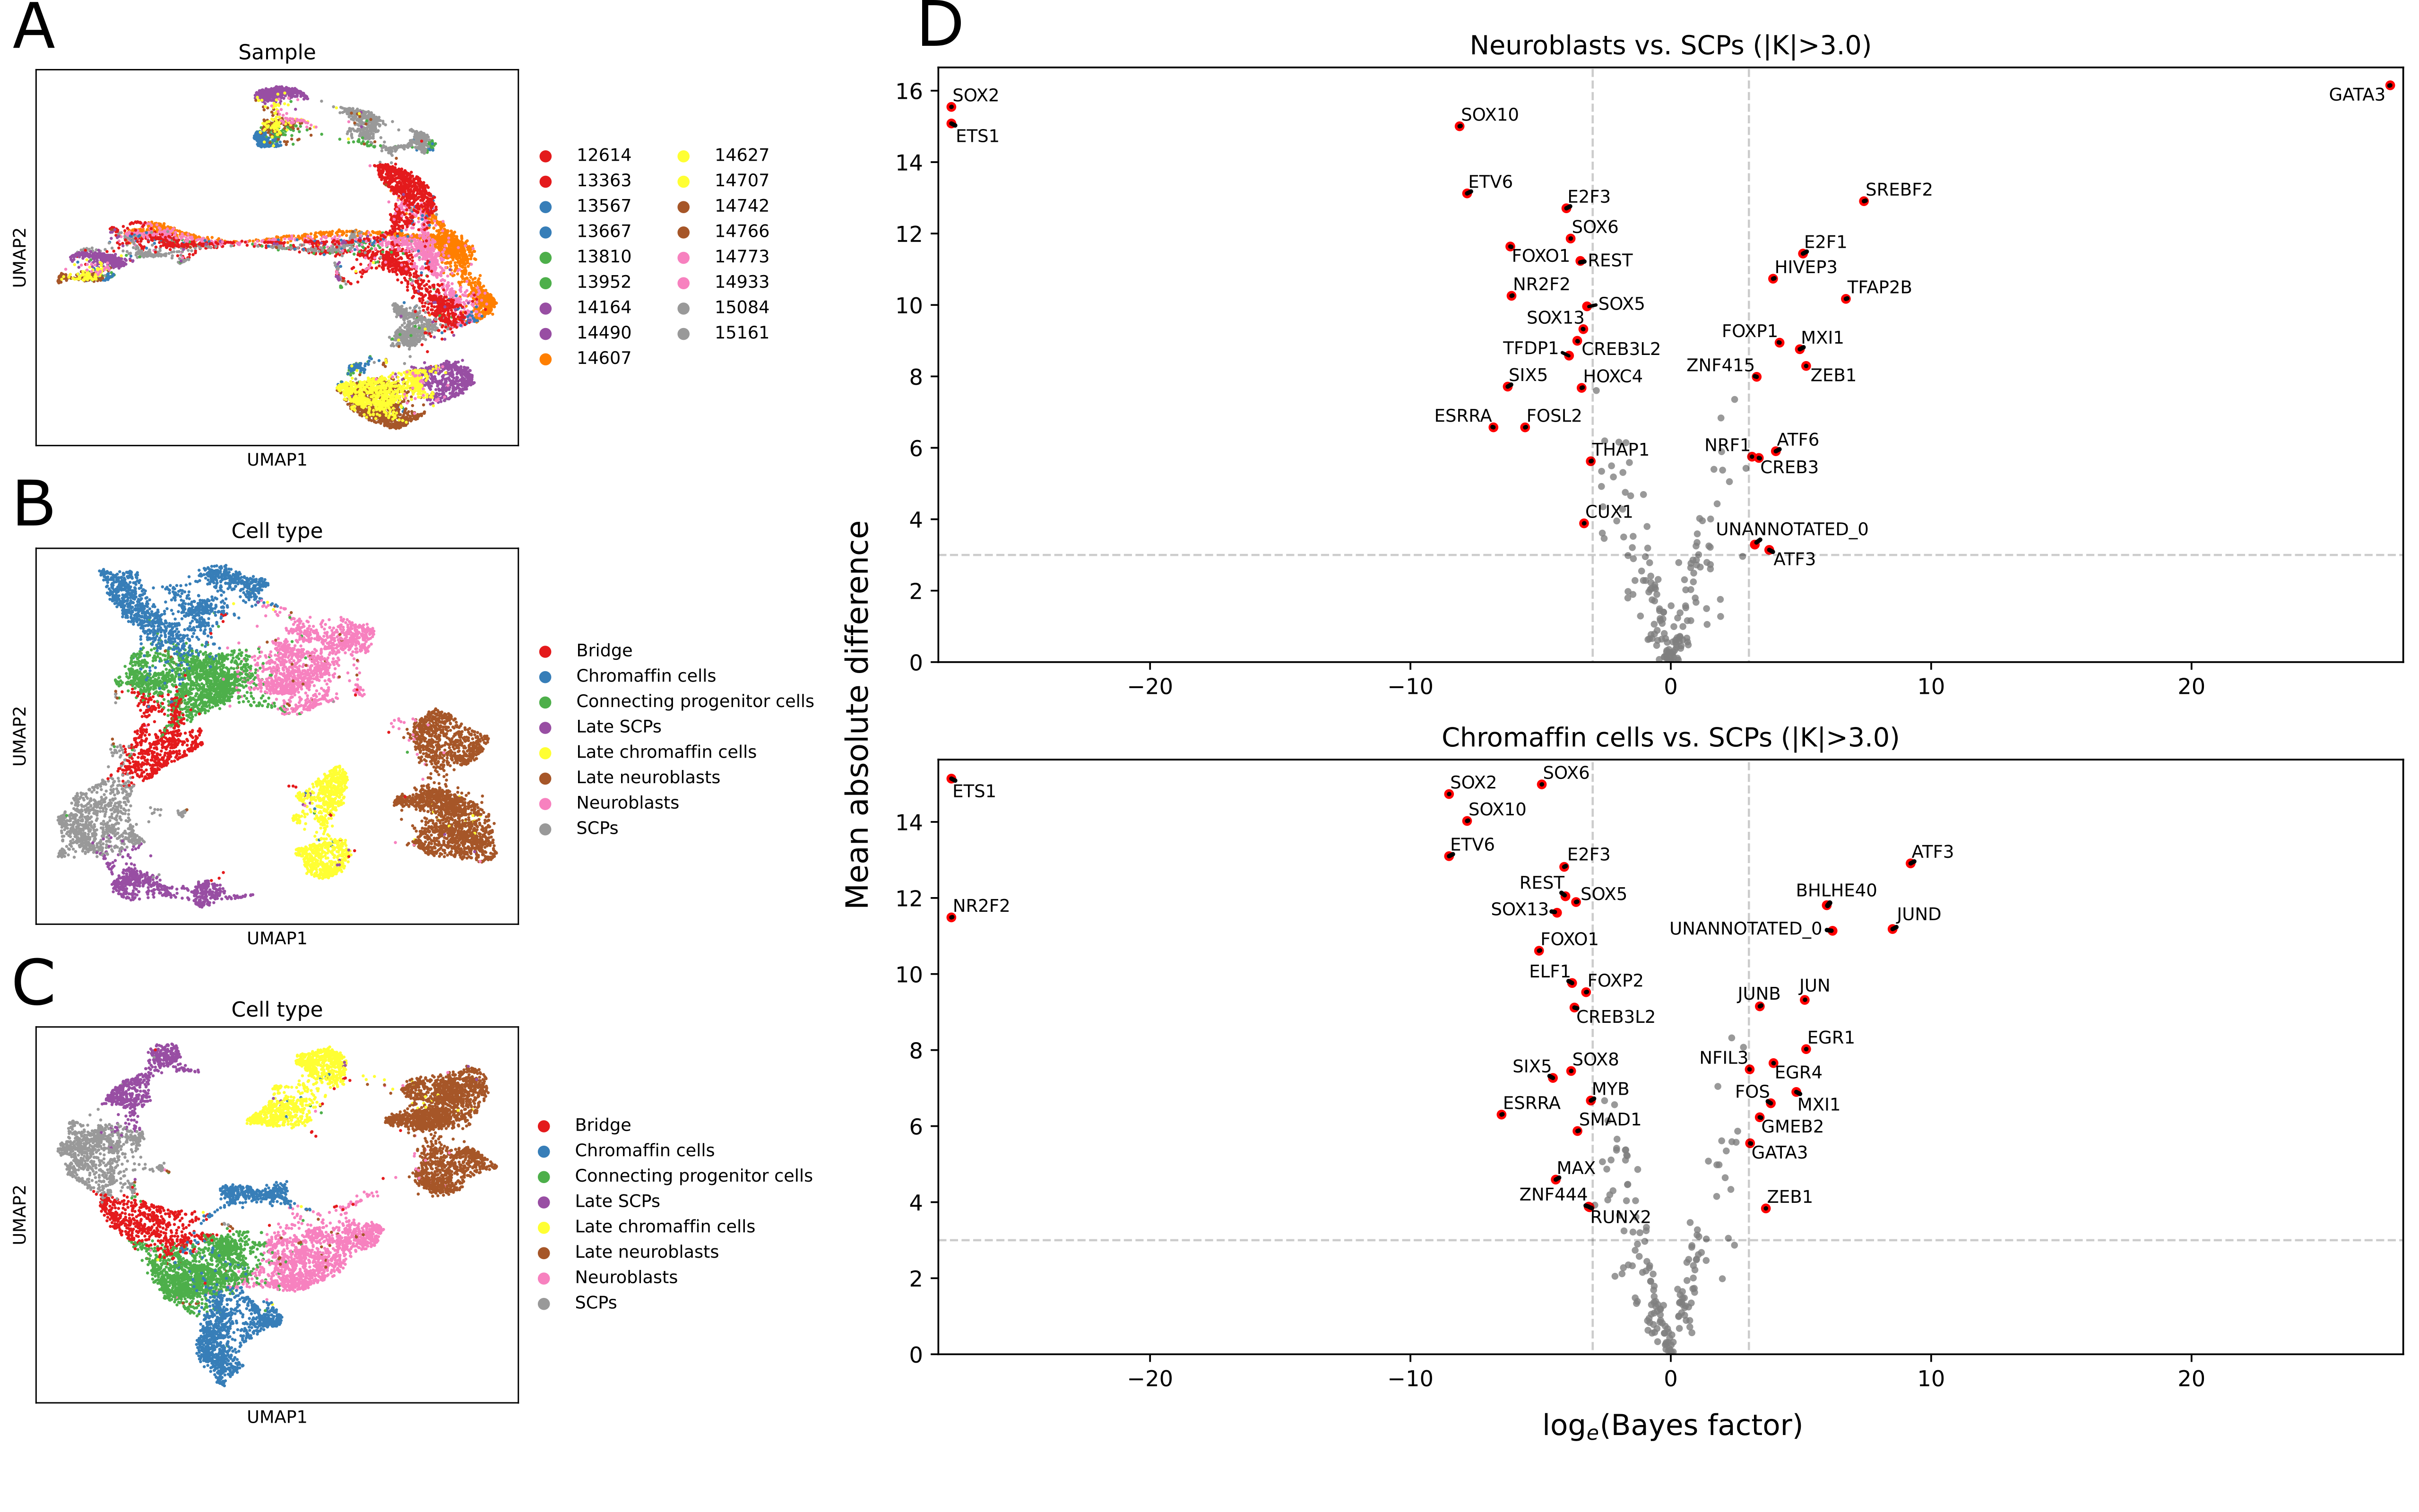
\includegraphics[scale=0.72]{SCENIC_sparse/adm_scenic_hvg_sparse_appx.png}
    \caption{\small{\textbf{Benchmarks for VEGA} | We used the SCENIC regulons inferred from the human adrenal medulla dataset as the prior to analyze TF activities of human adrenal medullary cells. \textbf{(A)} The UMAP embedding of the gene expression space of the adrenal medulla dataset colored by samples supports that the cell clustering was based on biological differences between the cell types rather than technical differences between the samples. \textbf{(B,C)} The UMAP embeddings of the VEGA latent spaces from the models trained on the datasets with the whole gene features and with only those genes connected to the GMVs according to the prior regulons. The UMAP plots show that the model could cluster cells into cell types but the developmental trajectories of the adrenal medulla were not preserved as well as using the dataset with the top 2000 highly variable genes. \textbf{(D)} The x-axis and the y-axis indicate the significance level and the mean absolute difference of GMV activity comparisons between two cell types. These volcano plots annotate all significantly differential TF activities for Fig.\ref{fig:sparse_adm_scenic}D for future use. We considered TFs to be significantly differentially activated when $|\textnormal{log}_e(\textnormal{BF})|>3$.}}
    \label{fig:sparse_adm_scenic_appx}
\end{figure}

\begin{figure}[h!]
    \centering
    \hspace*{-17mm}
    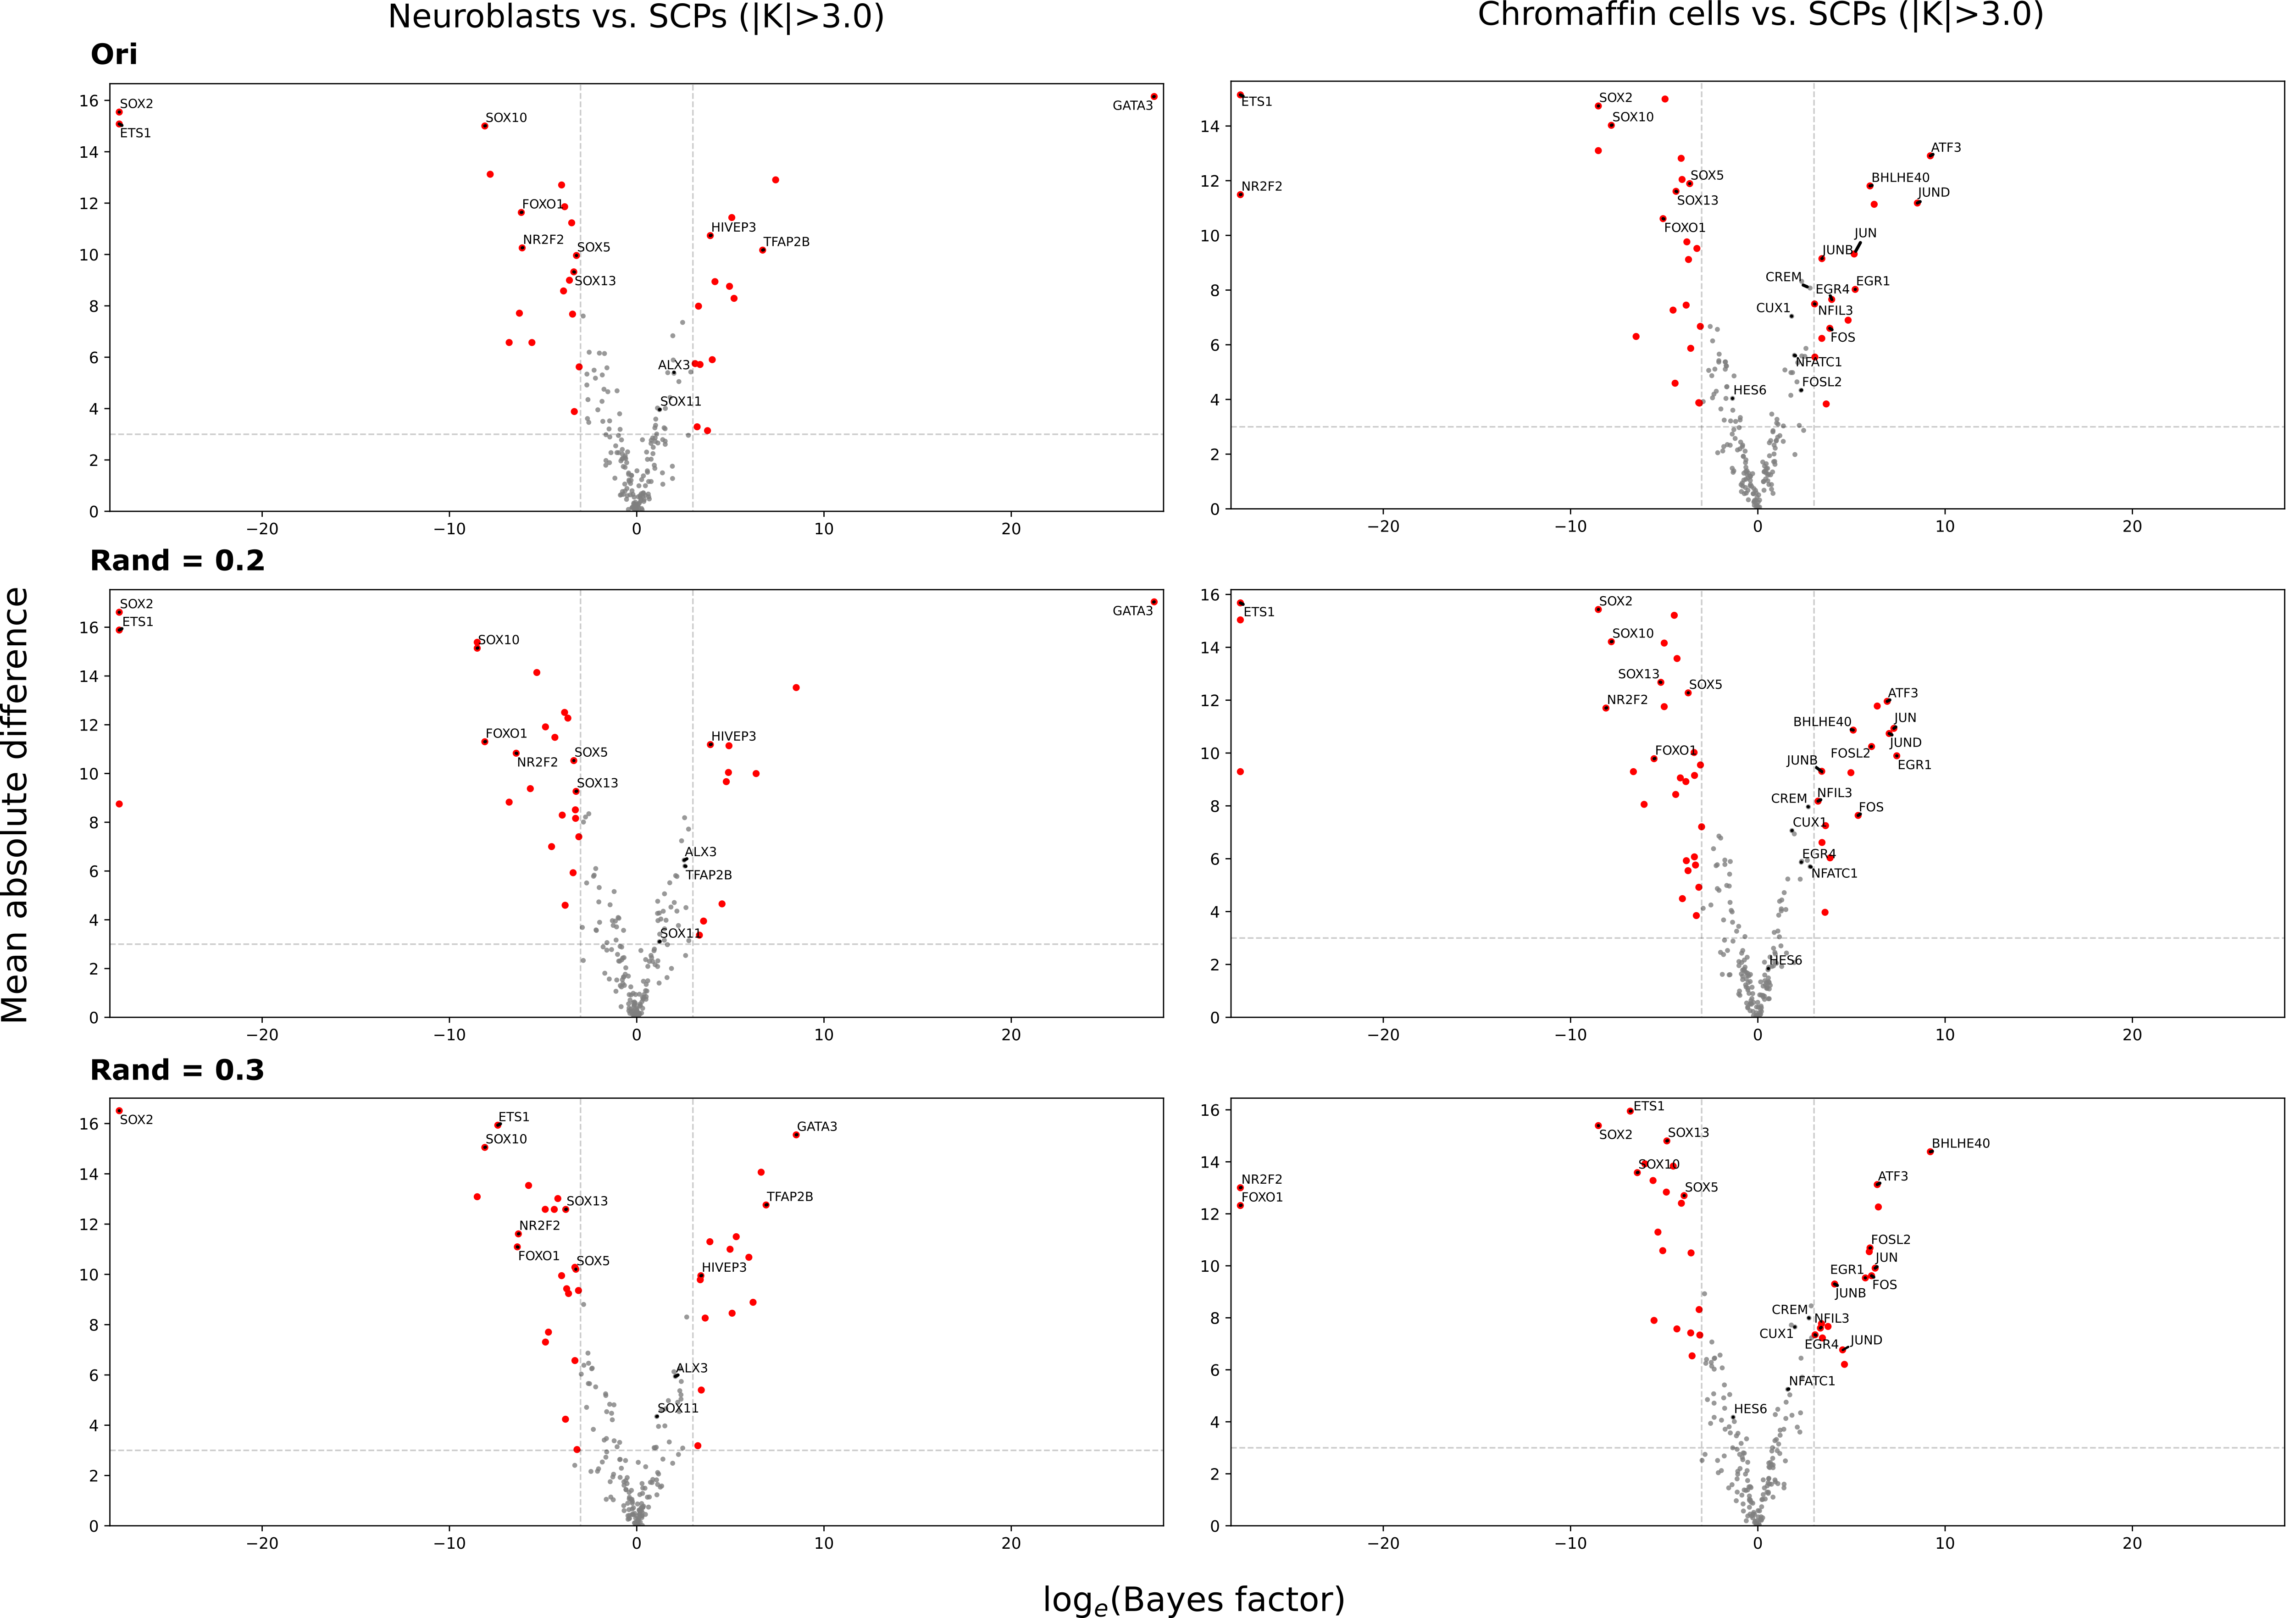
\includegraphics[scale=0.82]{SCENIC_sparse/adm_rand_hvg_appx.png}
    \caption{\small{\textbf{Changes in model interpretability when randomizing prior to different degrees} | The x-axis and the y-axis indicate the significance level and the mean absolute difference of GMV activity comparisons between two cell types. This figure is to complete the results of differential activity analysis on the VEGA embeddings using the prior which was randomized on different levels for Fig.\ref{fig:sparse_adm_rand_hvg2}. Rand indicates the degree of randomization of the prior. We considered TFs to be significantly differentially activated when $|\textnormal{log}_e(\textnormal{BF})|>3$. The rest of the results is on the next page.}}
    \label{fig:sparse_adm_rand_hvg_appx}
\end{figure}

\addtocounter{figure}{-1}
\begin{figure}[h!]
    \centering
    \hspace*{-17mm}
    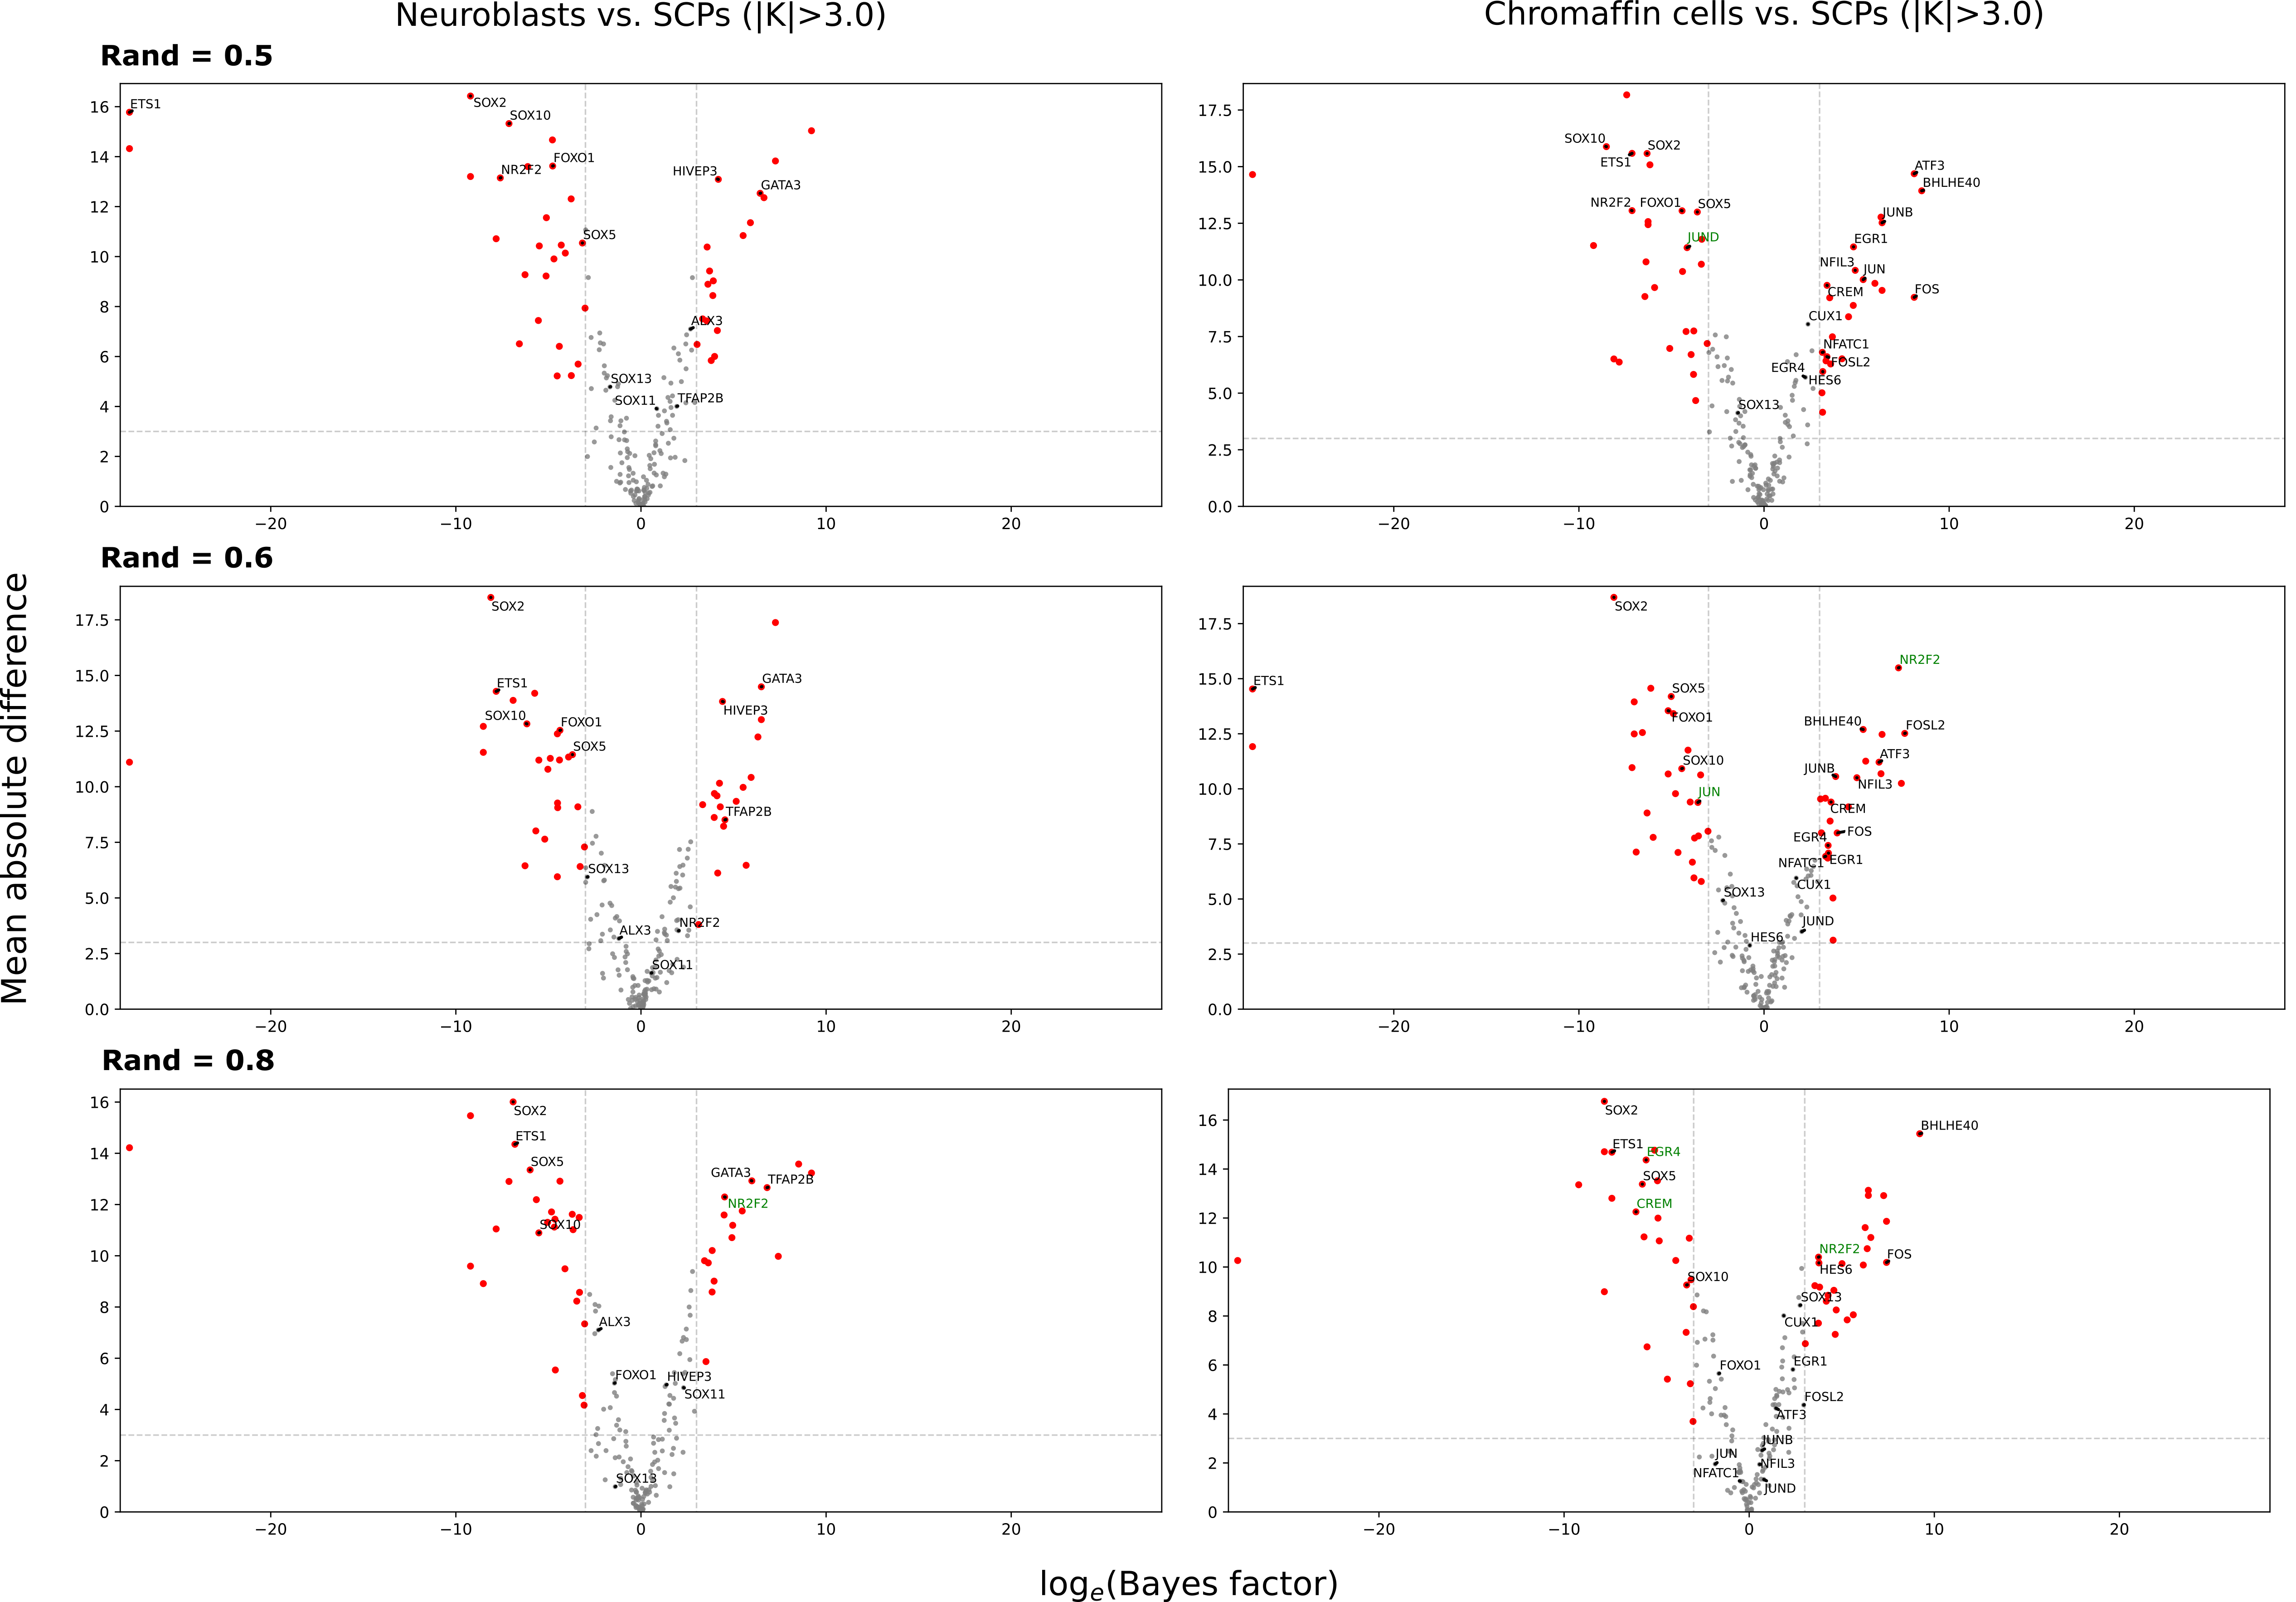
\includegraphics[scale=0.82]{SCENIC_sparse/adm_rand_hvg_appx2.png}
    \caption{\small{This figure is continued from the previous page.}}
\end{figure}

\begin{figure}[h!]
    \centering
    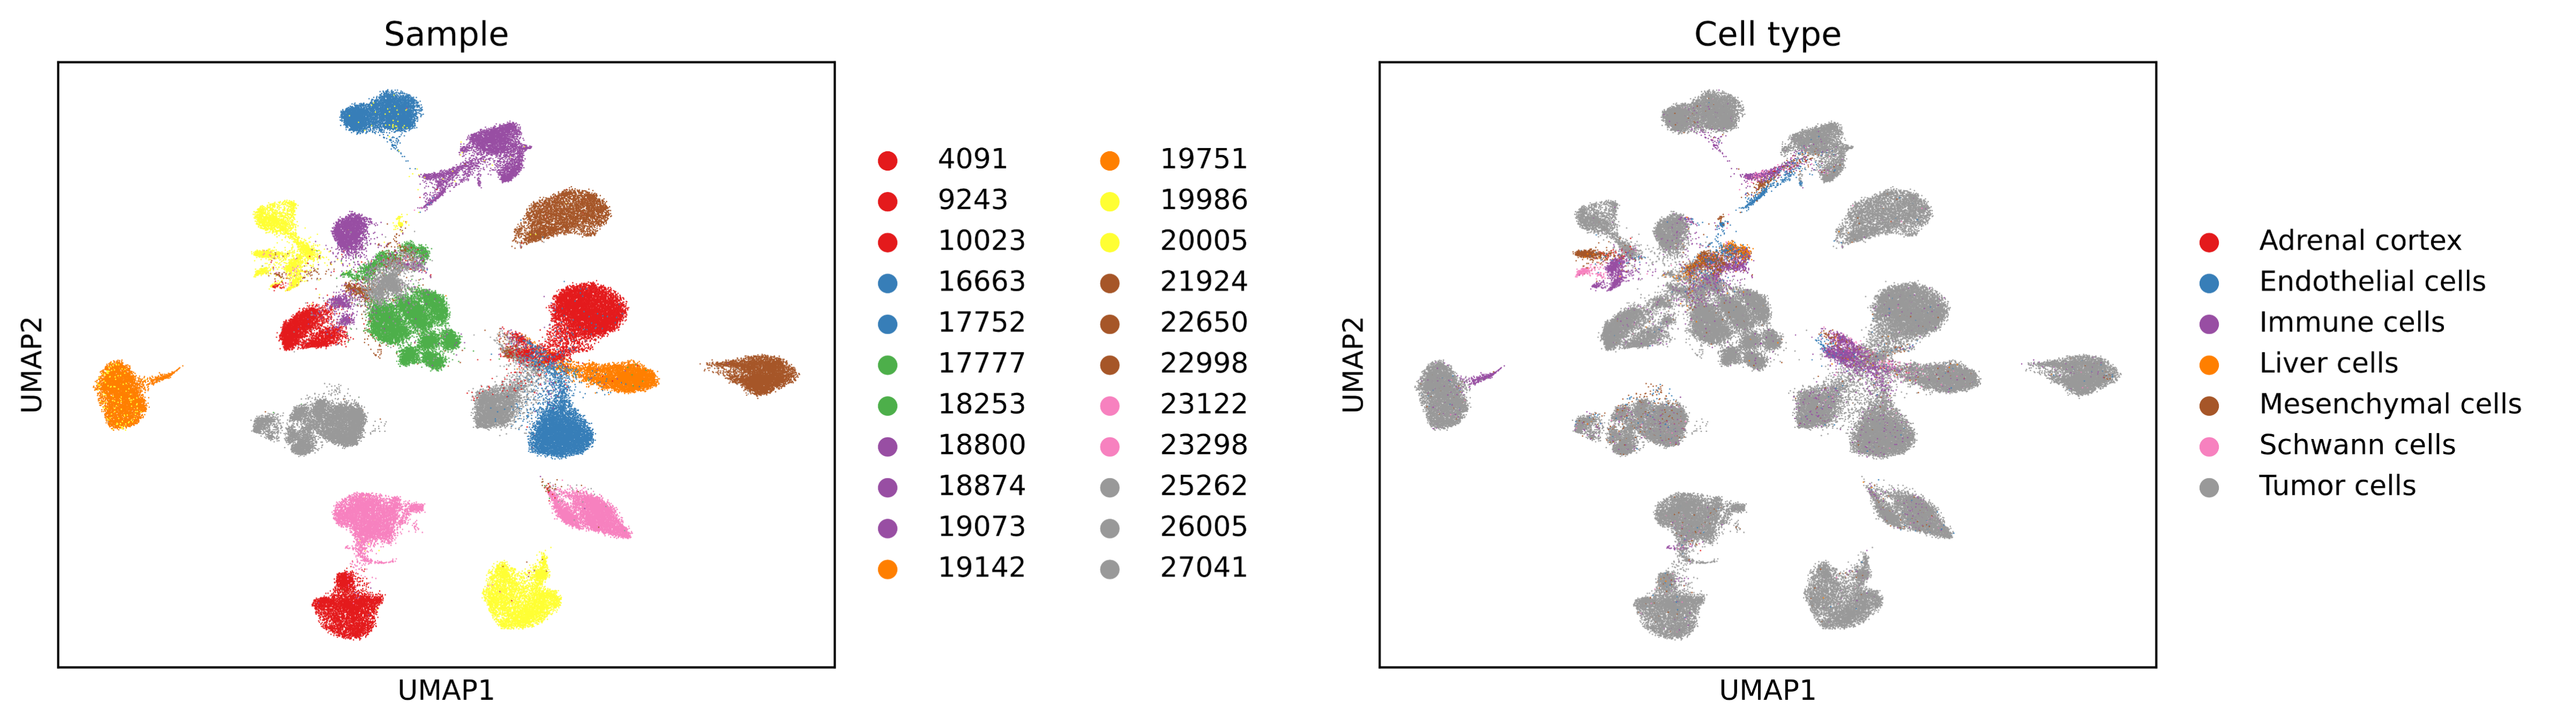
\includegraphics[scale=0.76]{SCENIC_sparse/nb_batch_appx.png}
    \caption{\small{\textbf{Testing of batch correction function of VEGA} | To verify that incorporating batch information in the model training is effective in alleviating batch effects, we trained the model with all the same settings as Fig.\ref{fig:sparse_nb_batch}B except incorporating the batch annotations. Without providing the batch annotations for the model training, the UMAP embedding of the VEGA latent space shows that cells were clustered mainly due to technical differences between the samples rather than biological differences between the cell types.}}
    \label{fig:sparse_nb_batch_appx}
\end{figure}

\begin{figure}[b!]
    \vspace{4cm}
    \caption{\small{\textbf{Investigation of regularized decoder behavior} | \textbf{(A)} The x-axis indicates the top 20 high-ranking genes (highest weights) of GATA3 from the hard-coded decoder of VEGA and the y-axis indicates the weight magnitude. This plot is to exhibit how we selected three artificially removed genes (prefixed by double asterisks). \textbf{(B)} The x-axis indicates the ranking of the weights of GATA3 and if the corresponding gene was annotated in the SCENIC GATA3 regulon, the frequency increased 1 in the y-axis. The recovery plot shows how the decoder behaved without using any prior knowledge (i.e., the decoder was fully connected). This is to support the finding that the regularized decoder behaves in a fully connected way when $\lambda\alpha$ is small. The red bar on a curve indicates the number of non-zero weights of GATA3 (i.e., the putative GATA3 regulon). Note that the zero-valued weights were randomly ranked. \textbf{(C)} The x-axis indicates the value of $\lambda\alpha$ and the y-axis indicates the number of non-zero weights of GATA3 (i.e., the putative GATA3 regulon). The plot shows that the number of putative target genes of GATA3 decreased when the model started using the prior evidently (from $\lambda\alpha = 10^{-3}$) and had a drastic drop when $\lambda\alpha$ was reaching 1. \textbf{(D,E)} Apart from GATA3, we also performed the same analyses on JUN to support the findings based on GATA3. Altogether, the results from JUN are very similar to those from GATA3, described in the caption of Fig.\ref{fig:L1_adm_removal}.}}
\end{figure}

\addtocounter{figure}{-1}
\begin{figure}[h!]
    \centering
    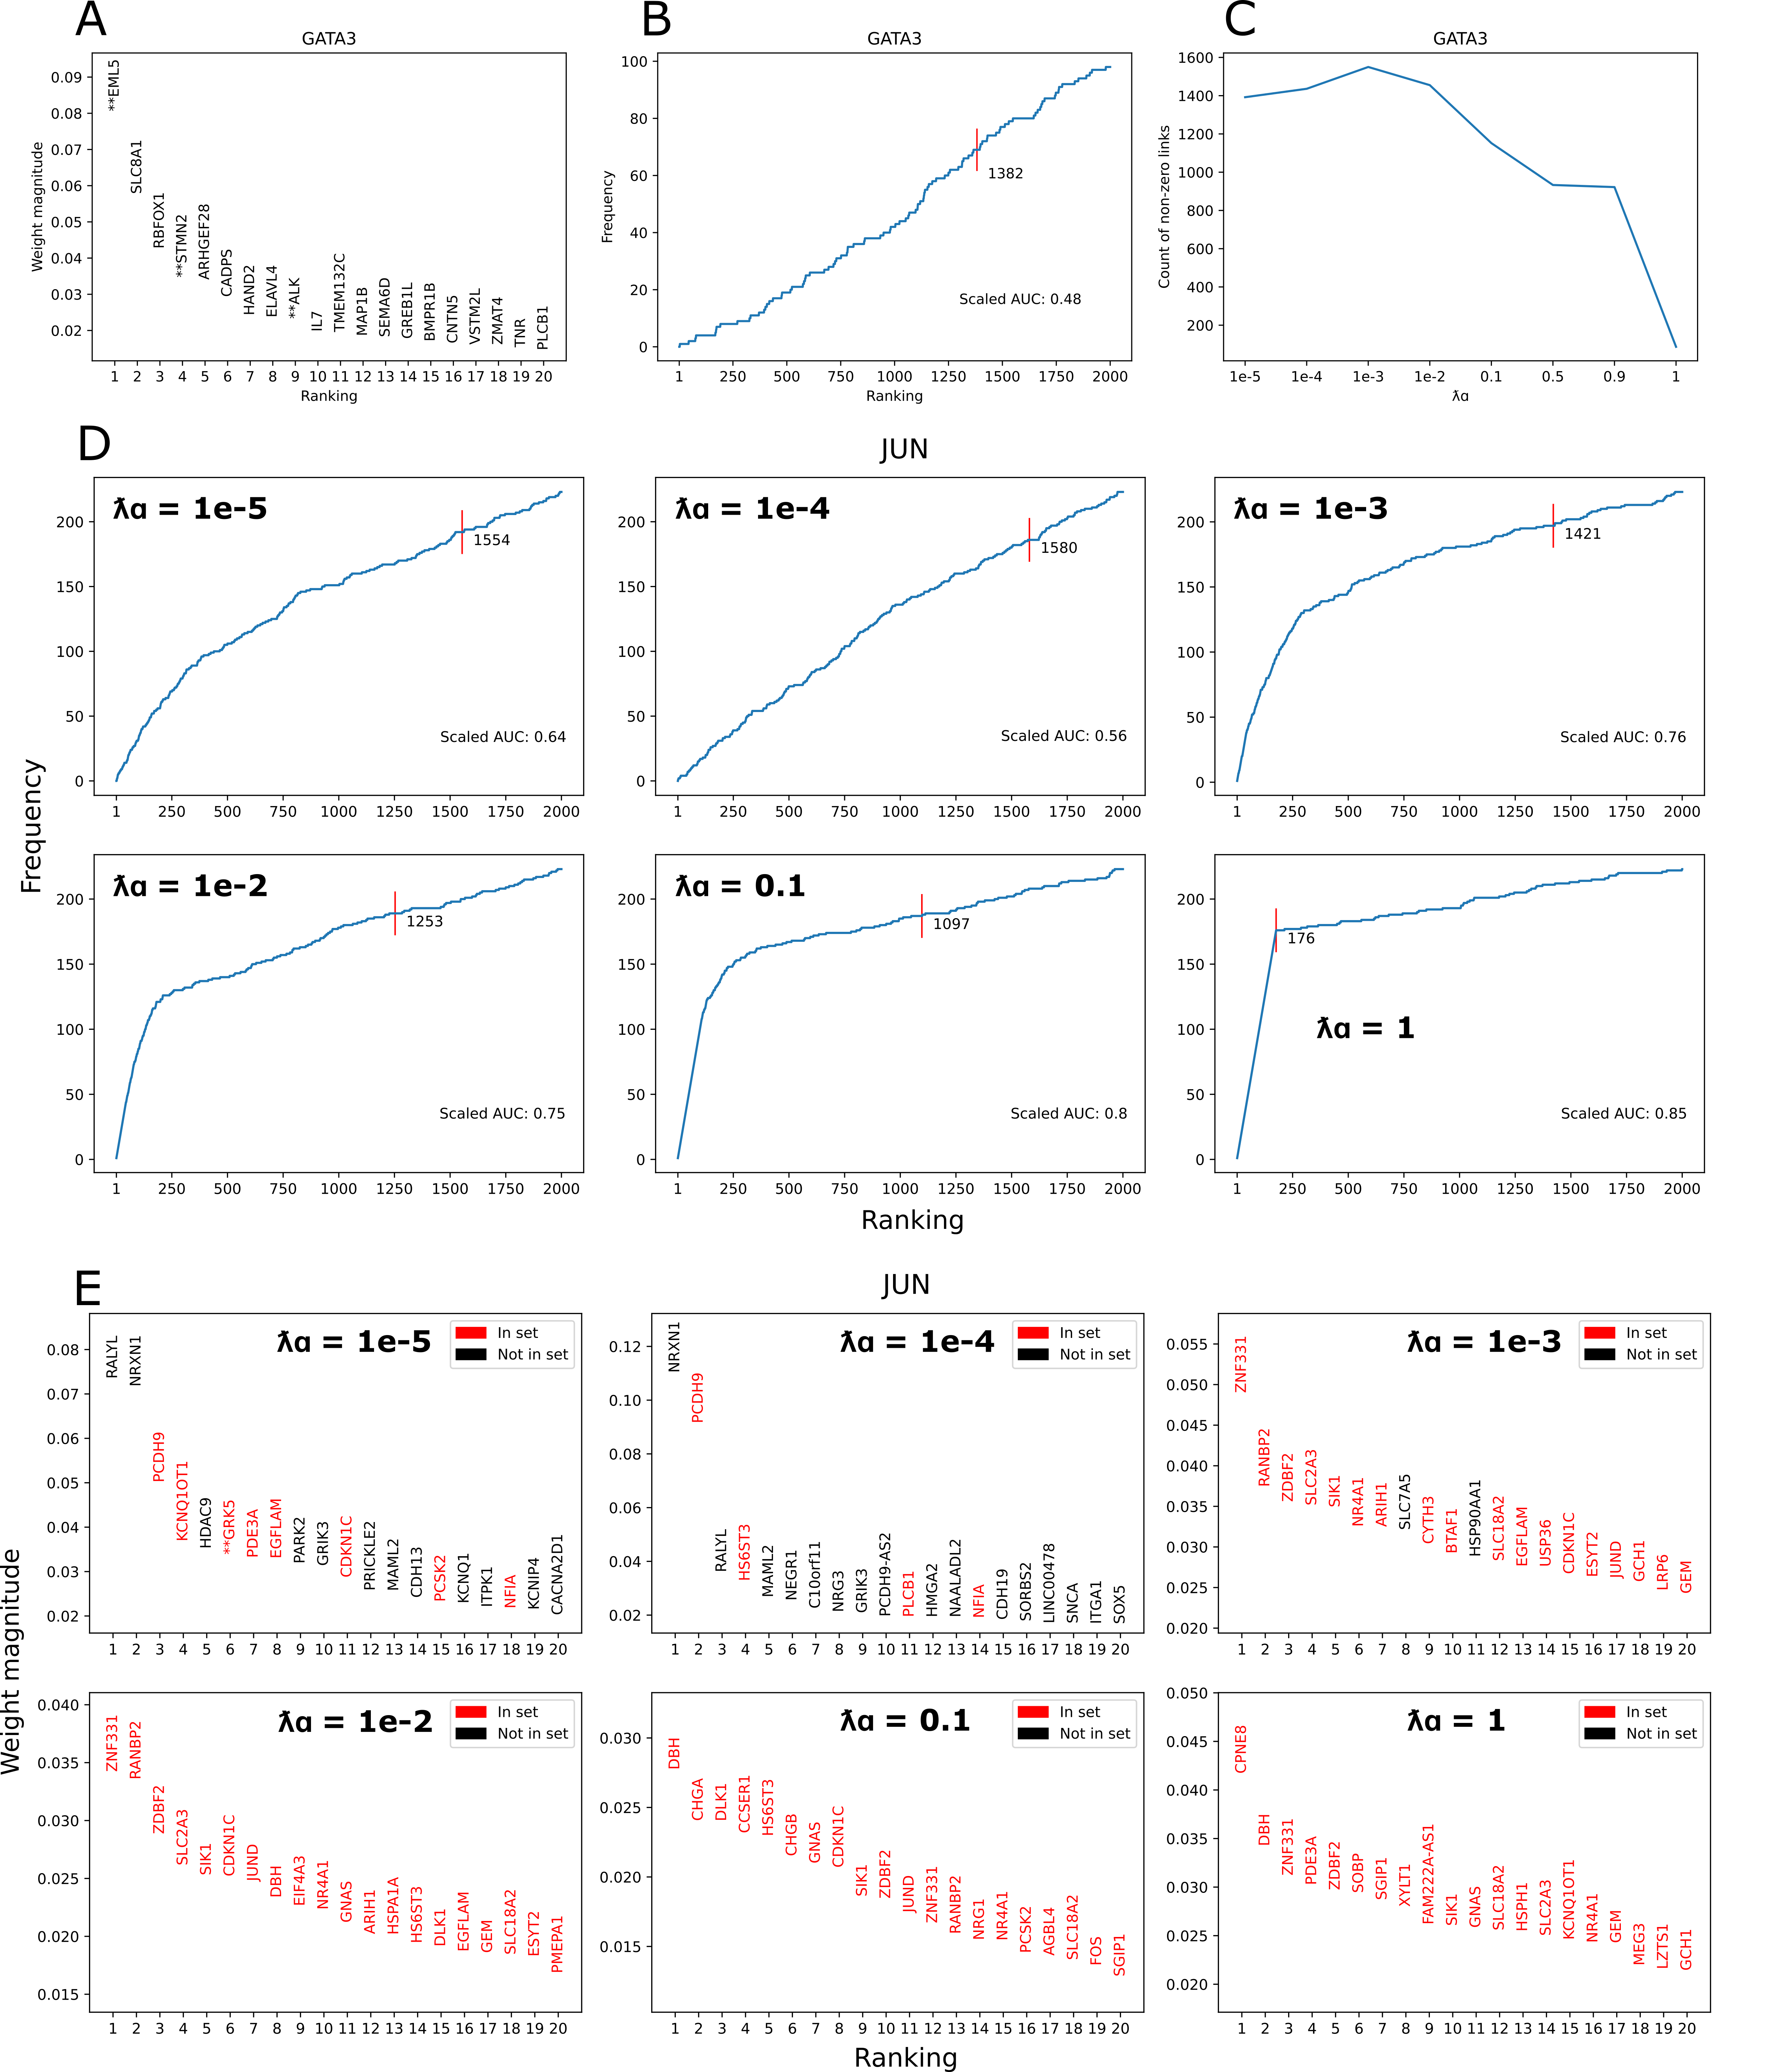
\includegraphics[scale=0.72]{SCENIC_L1/adm_L1_removal_appx.png}
    \caption{\small{The caption is on the previous page.}}
    \label{fig:L1_adm_removal_appx}
\end{figure}

\begin{figure}[h!]
    \centering
    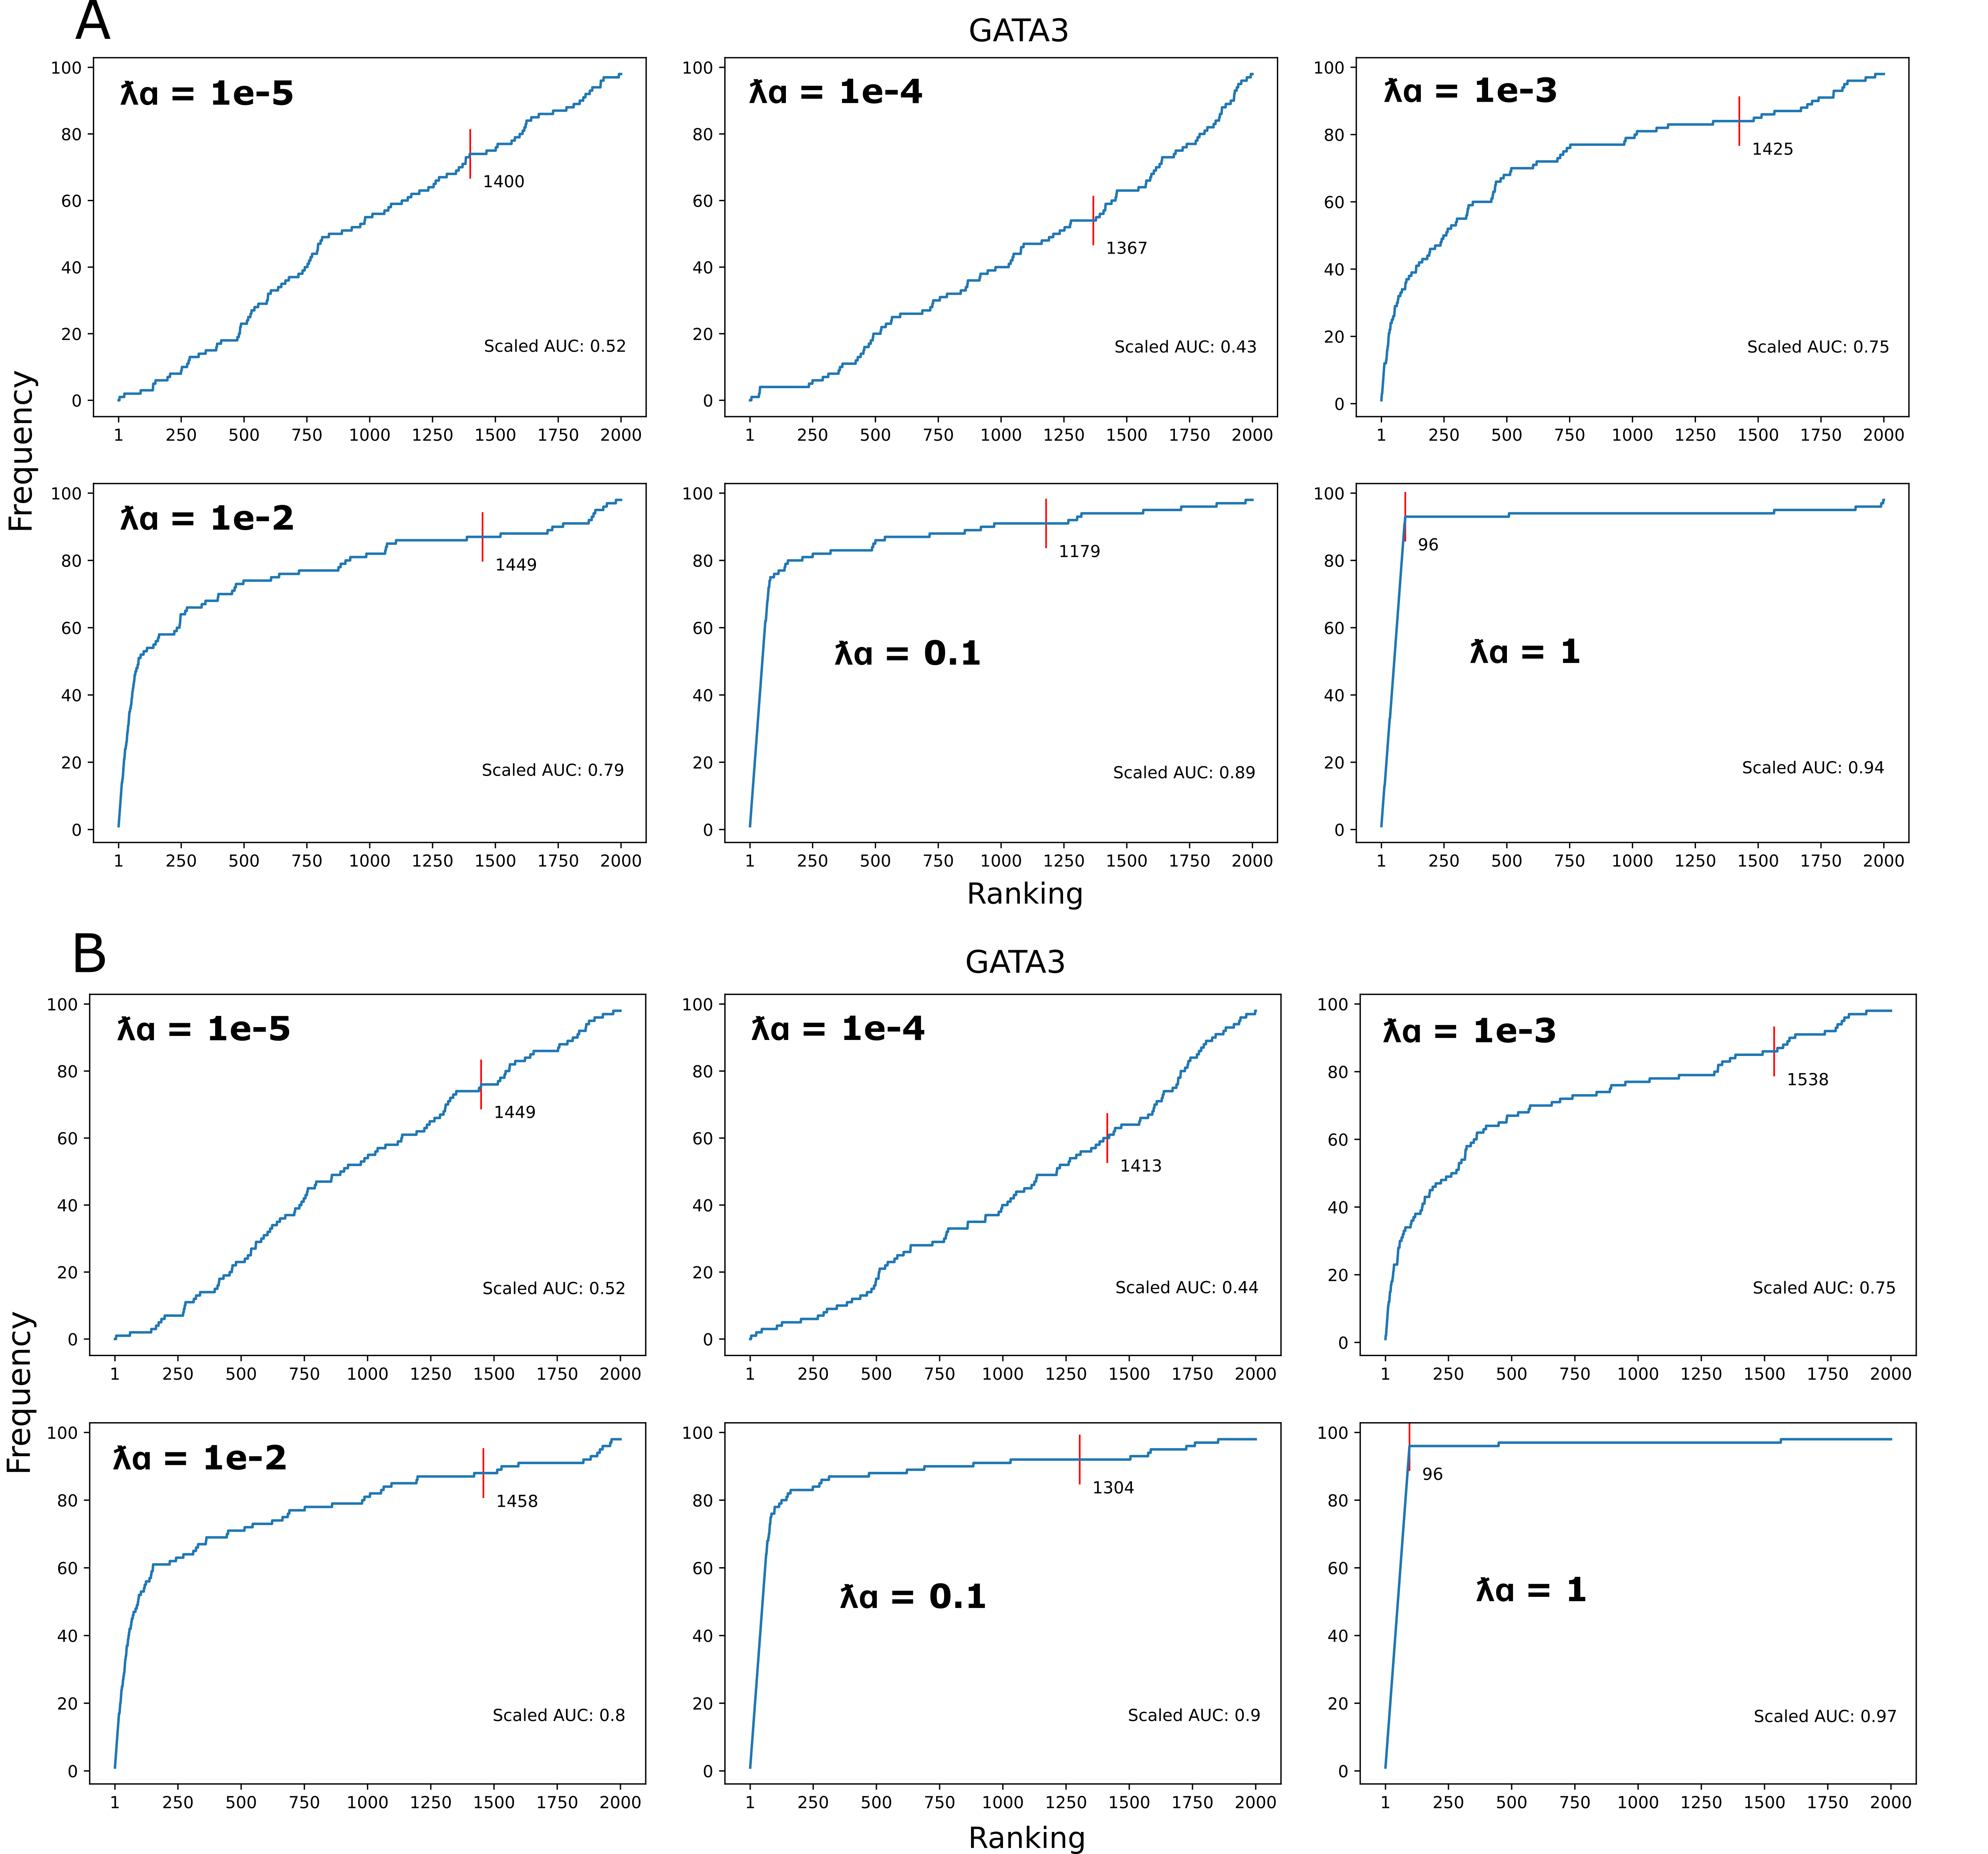
\includegraphics[scale=0.72]{SCENIC_L1/adm_L1_addition_appx.png}
    \caption{\small{\textbf{Results for supporting our findings on regularized decoder behavior} | The x-axis indicates the ranking of the weights of GATA3 and if the corresponding gene was annotated in the SCENIC GATA3 regulon, the frequency increased 1 in the y-axis. These recovery plots are to provide more evidence for our findings that the decoder behaves in a fully-connected way when $\lambda\alpha < 10^{-3}$, in a regularized way when $10^{-3} \leq \lambda\alpha <1$, in a hard-coded way when $\lambda\alpha = 1$ (Fig.\ref{fig:L1_adm_removal}A). \textbf{(A,B)} The difference between panel A and B lies in the SCENIC regulons we used as the prior where GATA3 was added with three genes with high average expression levels in panel A and with low average expression levels in panel B. The overall decoder behavior is not influenced by slightly artificially modified prior knowledge.}}
    \label{fig:L1_adm_addition_appx}
\end{figure}

\begin{figure}[h!]
    \centering
    \hspace*{-5mm}
    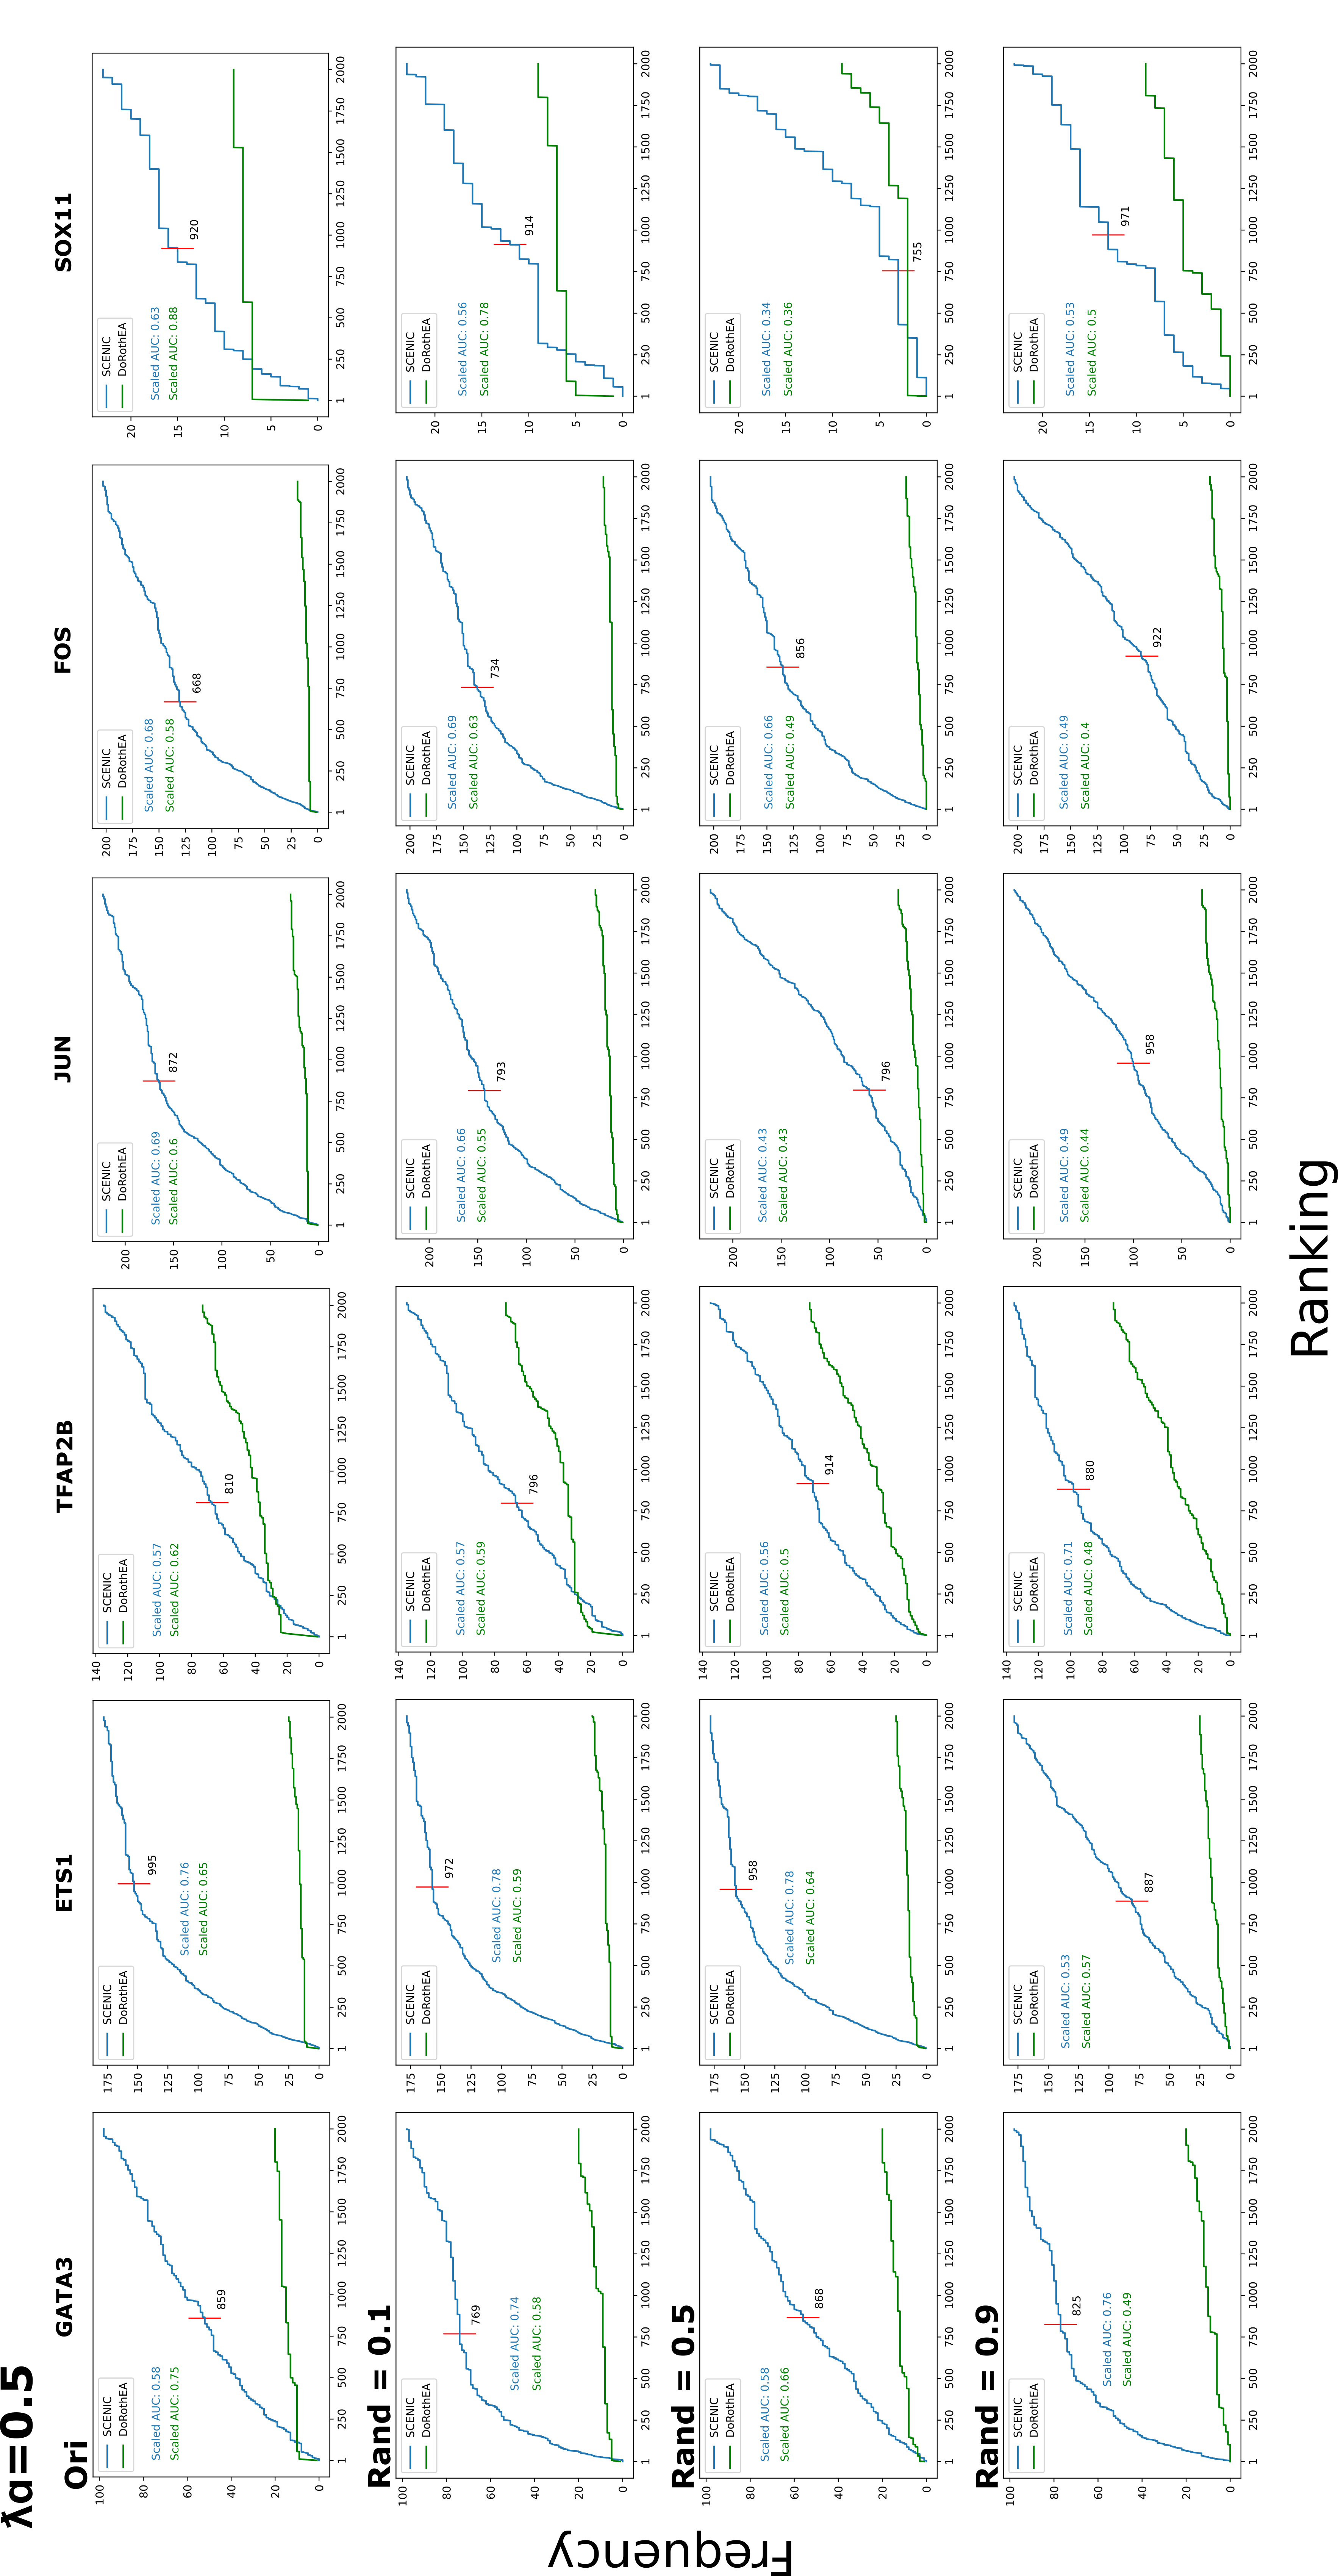
\includegraphics[scale=0.67]{DoRothEA_L1/adm_dorothea_L1_0.5_hvg_rand.png}
    \caption{\small{The caption is on the next page.}}
    \label{fig:L1_adm_dorothea_rand_0.5_hvg}
\end{figure}

\addtocounter{figure}{-1}
\begin{figure}[t!]
    \caption{\small{\textbf{Sanity check on prior knowledge randomization testing} | This figure is to provide more evidence for that the incorrect prior worsen the inference performance of the regularized decoder. Instead of using the model with $\lambda\alpha = 0.9$, we used the model with $\lambda\alpha = 0.5$ to investigate the changes in the dataset-specific GRN inferences when the non-context-specific DoRothEA regulons were randomized to varied degrees. The x-axis indicates the ranking of weights of a certain TF and if the corresponding gene was annotated in the SCENIC regulon (blue curves) or in the DoRothEA regulon (green curves) of the TF, the frequency increased 1 in the y-axis. Note that we will focus on blue curves for observing the inference capacity changes. The columns and the rows show the different TFs and the different degrees of randomization of the prior. Similarly to the model with $\lambda\alpha = 0.9$, there was no evident pattern of the changes in the inference performance when the prior was 10\% and 50\% randomized and most of the GRN inferences, except GATA3 and TFAP2B, were lost when the prior was 90\% randomized. The red bar on a curve indicates the number of non-zero weights of a certain TF (i.e., the putative regulon of the TF). Note that the zero-valued weights were randomly ranked. Ori indicates the original prior and Rand indicates the degree of randomization of the prior.}}
\end{figure}

\begin{figure}[b!]
    \vspace{4cm}
    \caption{\small{\textbf{Overview of inference capacity of regularized decoder across different $\lambda\alpha$} | We trained the model with the regularized decoder on the human adrenal medulla dataset and using the non-context-specific DoRothEA regulons as prior knowledge to infer more dataset-specific regulons. We computed AUC scores on recovery curves generated from decoder weights of each GMV based on the SCENIC adrenal medulla regulons to study the inference capacity of the regularized decoder. We display the AUC scores of each GMV (TF) from the individual models with different $\lambda\alpha$ values via heatmaps to provide a general picture of the changes in the inference capacity across different values of $\lambda\alpha$ used. The column and the row indicate the $\lambda\alpha$ values and the TFs. The result shows that, with different $\lambda\alpha$ values, the overall inference capacity of the regularized decoder did not differ much. This was proved by computing the median of the AUC scores from each column, where $\lambda\alpha = 10^{-3}$ is 0.53, $\lambda\alpha = 10^{-2}$ is 0.52, $\lambda\alpha = 0.1$ is 0.53, $\lambda\alpha = 0.5$ is 0.53, $\lambda\alpha = 0.9$ is 0.51 and $\lambda\alpha = 1$ is 0.48. Besides, a majority of TFs were not precisely inferred to more dataset-specific regulons and there was no clear pattern of how the regularized decoder treats the individual TFs with different $\lambda\alpha$ values. Interestingly, the top white block containing zero-valued AUC scores including all GMVs without any connection to the genes in the output layer, which indicates the model with the regularized decoder can exclude these GMVs that may hold wrong information automatically.}}
\end{figure}

\addtocounter{figure}{-1}
\begin{figure}[h!]
    \centering
    \hspace*{-6mm}
    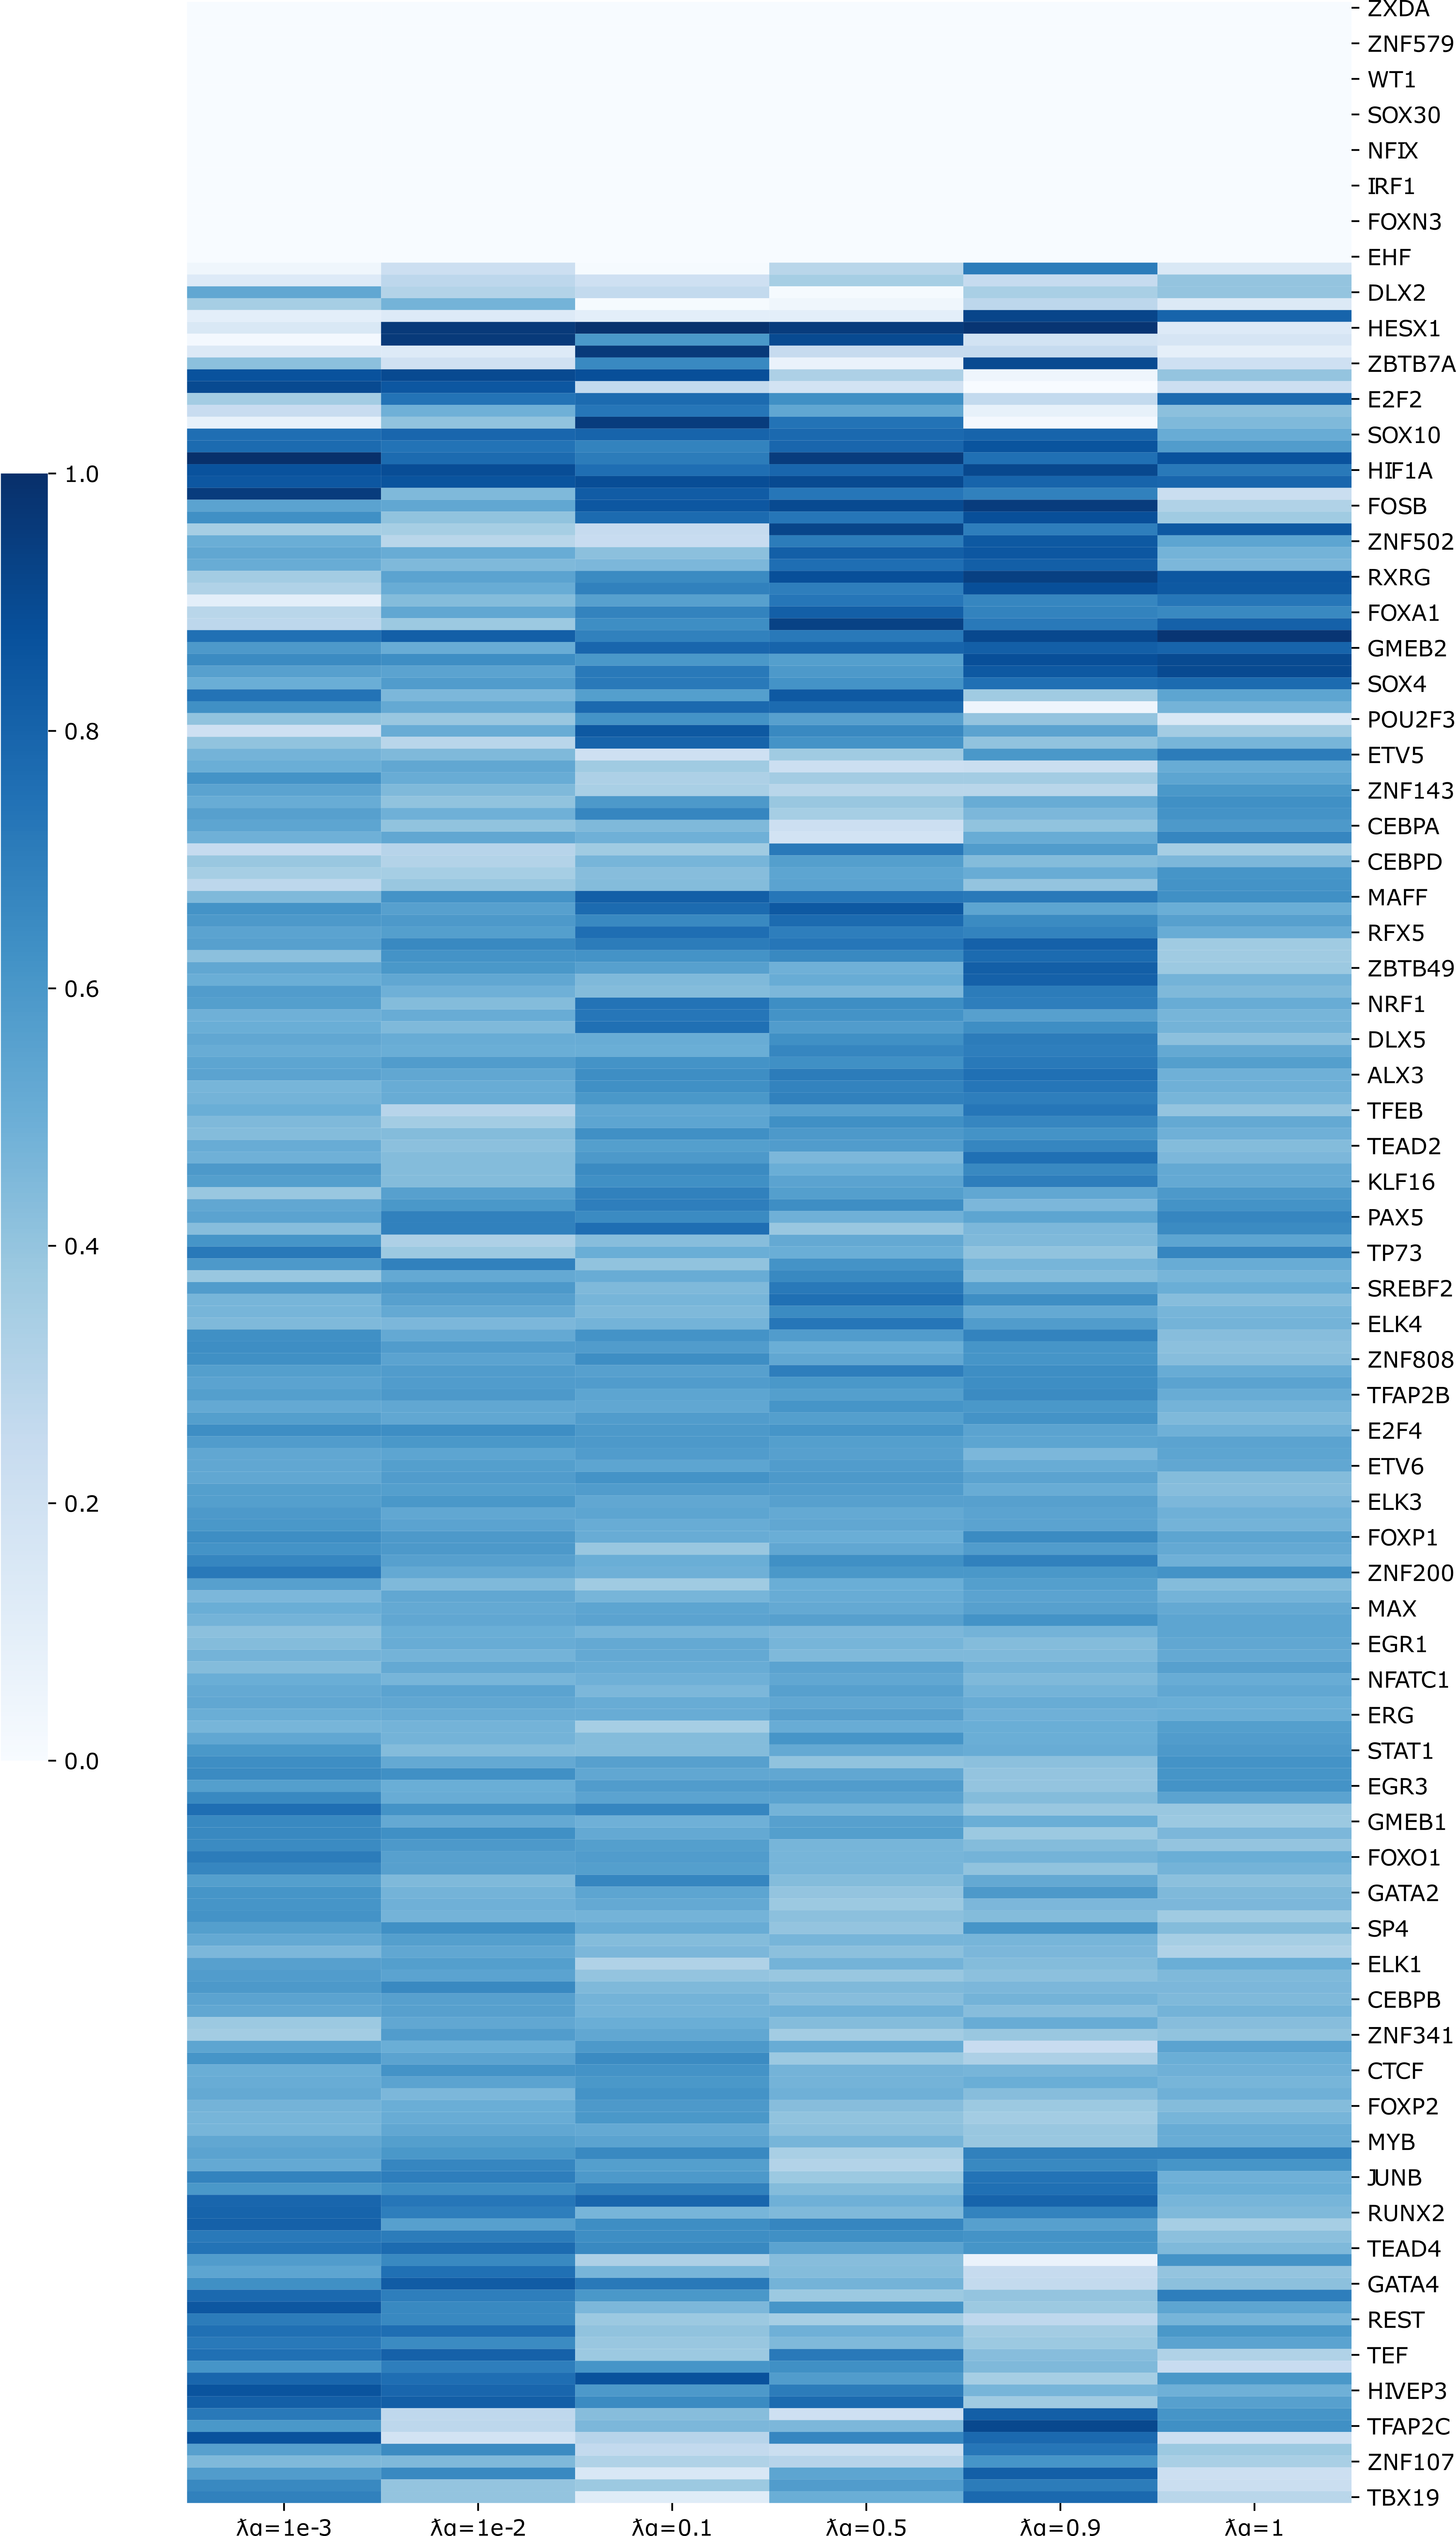
\includegraphics[scale=0.65]{DoRothEA_L1/scenic_heatmap.png}
    \caption{\small{The caption is on the previous page.}}
    \label{fig:L1_dorothea_scenic_heatmap}
\end{figure}
